\documentclass[8pt]{beamer}

\mode<presentation>
{
  \usetheme{Warsaw}       % or try default, Darmstadt, Warsaw, ...
  \usecolortheme{dolphin} % or try albatross, beaver, crane, ...
  \usefonttheme{serif}    % or try default, structurebold, ...
  \setbeamertemplate{navigation symbols}{}
  \setbeamertemplate{caption}[numbered]
} 

\usepackage[spanish]{babel}
\usepackage[utf8x]{inputenc}
\usepackage{wrapfig}
\usepackage[beamer,customcolors]{hf-tikz} %Para hacer los cuadraditos de colores en las ecuaciones.
\hfsetfillcolor{alerted text.fg!10}
\hfsetbordercolor{alerted text.fg}
\usepackage{subcaption} %Para el entorno subfiguras.
\usepackage{ragged2e} % Justificar.
\usepackage{bm}

% On Overleaf, these lines give you sharper preview images.
% You might want to `comment them out before you export, though.
\usepackage{pgfpages}
\pgfpagesuselayout{resize to}[physical paper width=8in, physical paper height=6in]

% Here's where the presentation starts, with the info for the title slide
\title[Rol del Eje de Simetría Quíntuple en TrV]{\textbf{Cálculos Computacionales en Macromoléculas: Rol del Eje de Simetría Quíntuple en el Virus del Triatoma (TrV). Comparación con otros Virus Icosaédricos.}}
\author{Juan Francisco Viso}
\institute{
\begin{minipage}{0.3\textwidth}
\flushright{
\includegraphics[scale=0.1]{Figure/UNS.jpg}}
\end{minipage}
\begin{minipage}{0.3\textwidth}
\centering
 Universidad Nacional del Sur \\ Instituto de Física del Sur 
\end{minipage}
\begin{minipage}{0.3\textwidth}

\includegraphics[scale=0.1]{Figure/ifisur.jpg}
\end{minipage}
}
\date{8 de Junio de 2018}

\begin{document}

\begin{frame}
  \titlepage
   \begin{center}
   \begin{minipage}{0.9\textwidth}
     \centering
     %\vspace{-1.2cm}
     \underline{Director} \hfill \underline{Co-Director} \\ Marcelo D. Costabel \hfill Diego Guérin
    \end{minipage}
  \end{center}
\end{frame}


\begin{frame}[t]
\hspace{-0.7cm}
\begin{minipage}[t]{0.6\textwidth}
\begin{itemize}
    \item ¿Que es un \textbf{Virus}? 
    \begin{itemize}
        \item Son pequeños agentes infectivos que dependen de otros organismos para reproducirse.
        \item Material genético + \textbf{Cápside} proteica.
        \item Proceso de infección $\rightarrow$ \textbf{Desconocido}. \vfill
    \end{itemize}
    \item<2-> \textbf{Cápside Viral}.
    \begin{itemize}
        \item<2-> Están compuestas por \textbf{proteínas}.
        \item<2-> Estructura \textbf{icosaédrica} o Helicoidal.
        \item<2-> Función $\rightarrow$ \textbf{Protección} e \textbf{Interacción durante el proceso de infección}.
    \end{itemize}
    \item<3-> \textbf{Proteínas}.
    \begin{itemize}
        \item<3-> Cadenas lineales de \textbf{aminoácidos}.
        \item<3-> Distintas funciones: enzimática, inmunológica, estructural, protectora, etc.
    \end{itemize}
    \item<4-> Proteínas de Membrana: \textbf{Canales Iónicos}.
    \begin{itemize}
        \item<3-> Gran importancia biológica: definir los potenciales de reposo en las membranas celulares, permitir el flujo de iones Ca$^2+$, controlar el volumen celular, etc.
        \item<3-> Mecanismo de regulación de su apertura: \textbf{Puerta Hidrofóbica}.
    \end{itemize}
\end{itemize}
\end{minipage}
\begin{minipage}[t]{0.4\textwidth}
\centering
\only<1>{\begin{figure}[ht]
    \centering
    \vspace{1cm}
    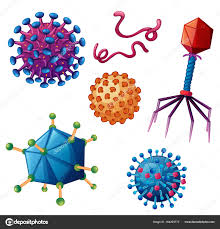
\includegraphics[width=0.9\textwidth]{Figure/virus.jpg}
\end{figure}}
\only<2>{\begin{figure}[ht]
    \centering
    \vspace{-0.5cm}
    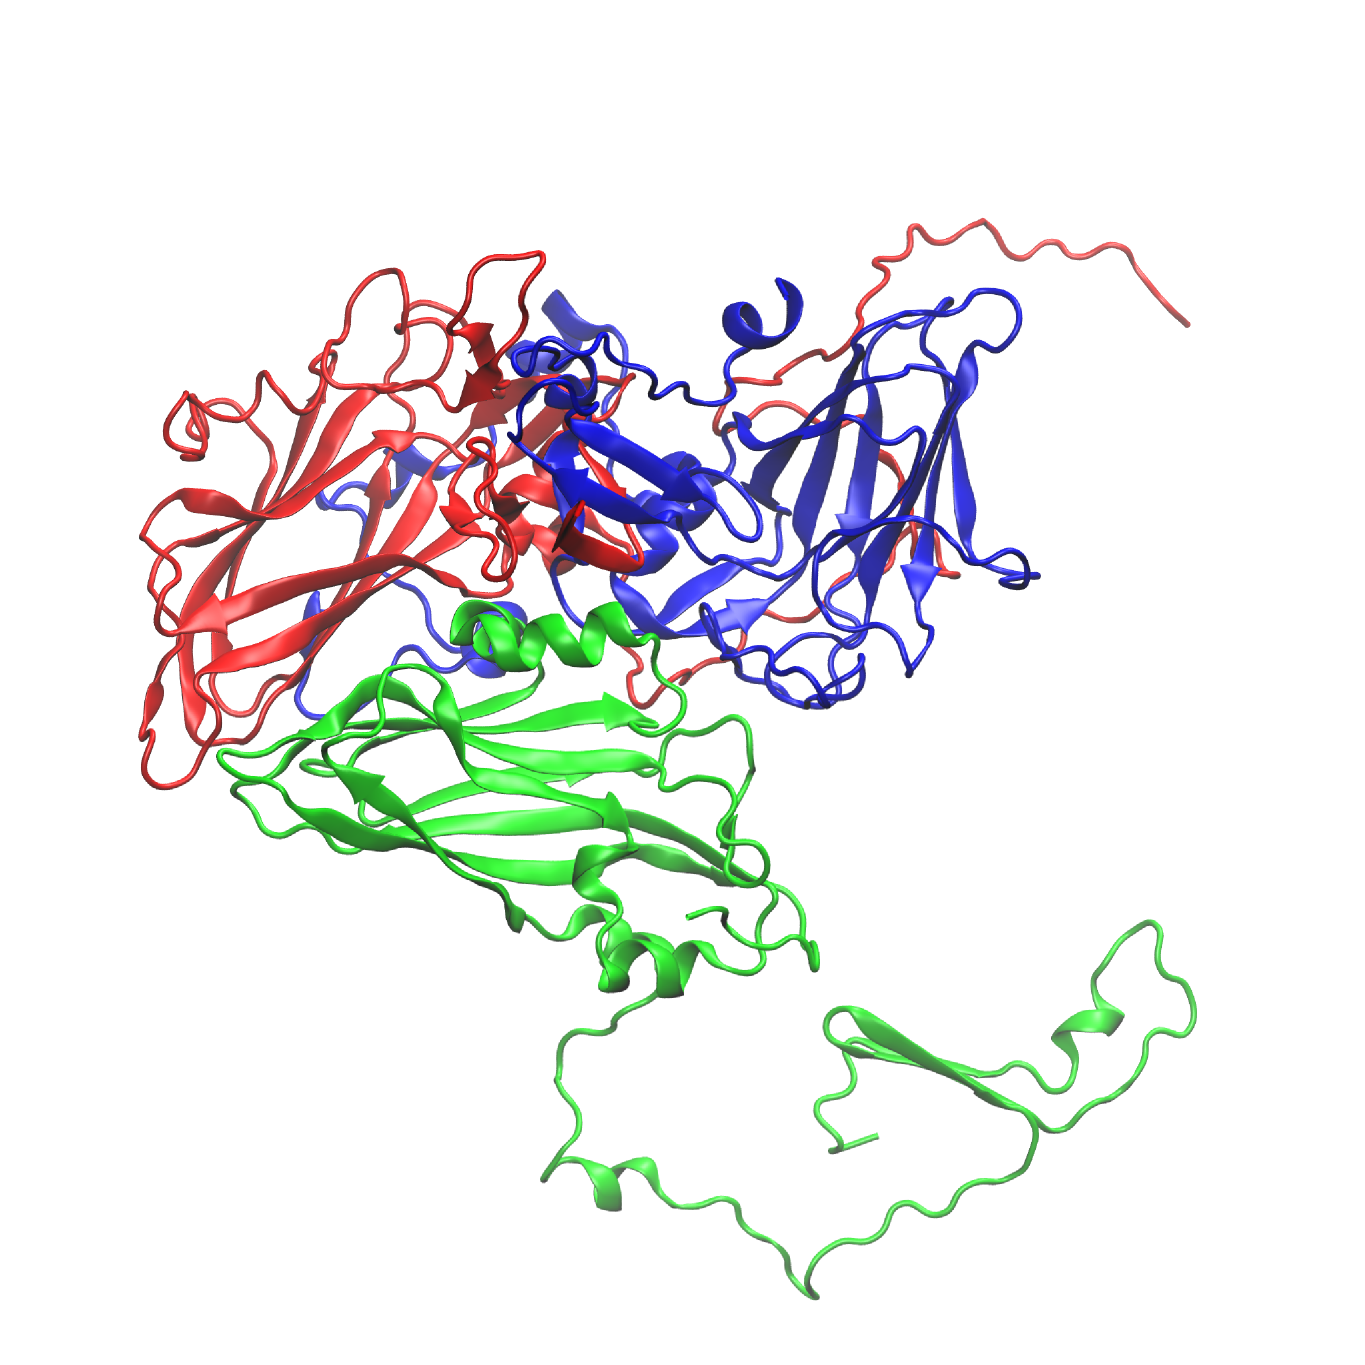
\includegraphics[width=0.9\textwidth]{Figure/TrV_Protomer.png}\\
    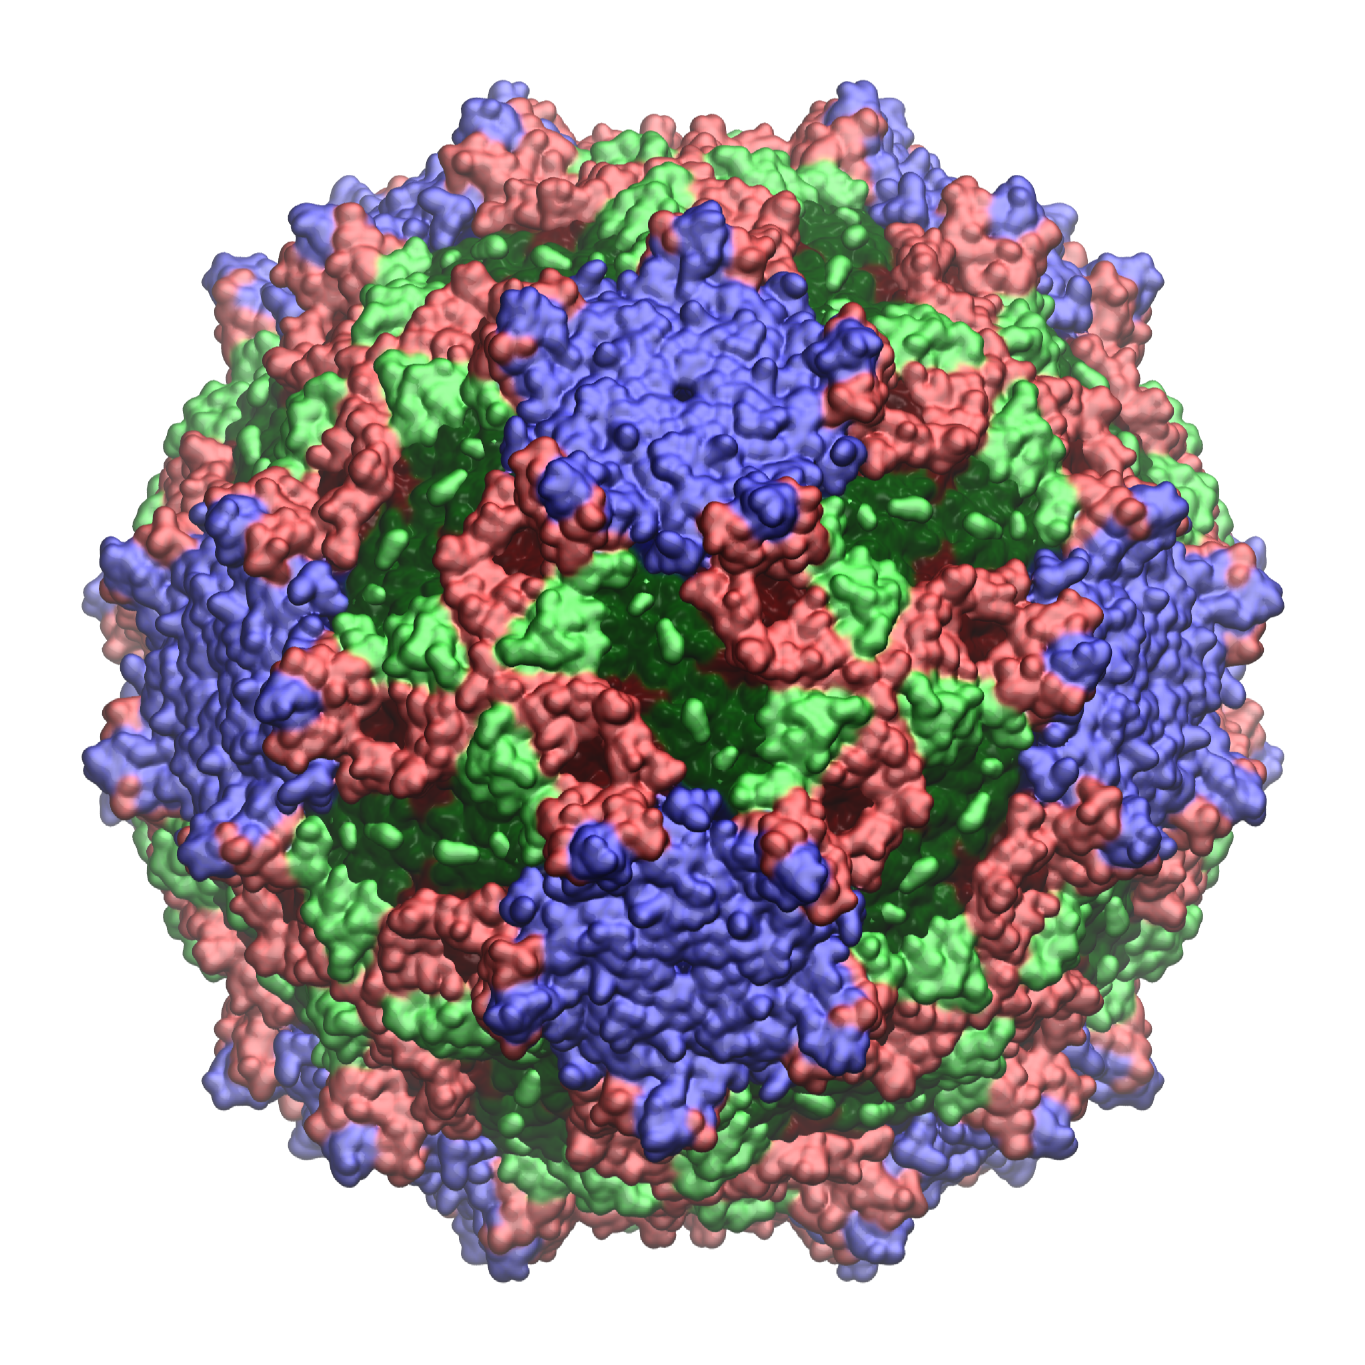
\includegraphics[width=0.9\textwidth]{Figure/TrV_Capsid.png}
\end{figure}}
\only<3>{\begin{figure}[ht]
    \centering
    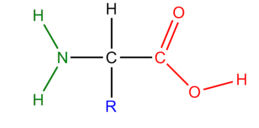
\includegraphics[width=0.9\textwidth]{Figure/aa.jpg}\\
    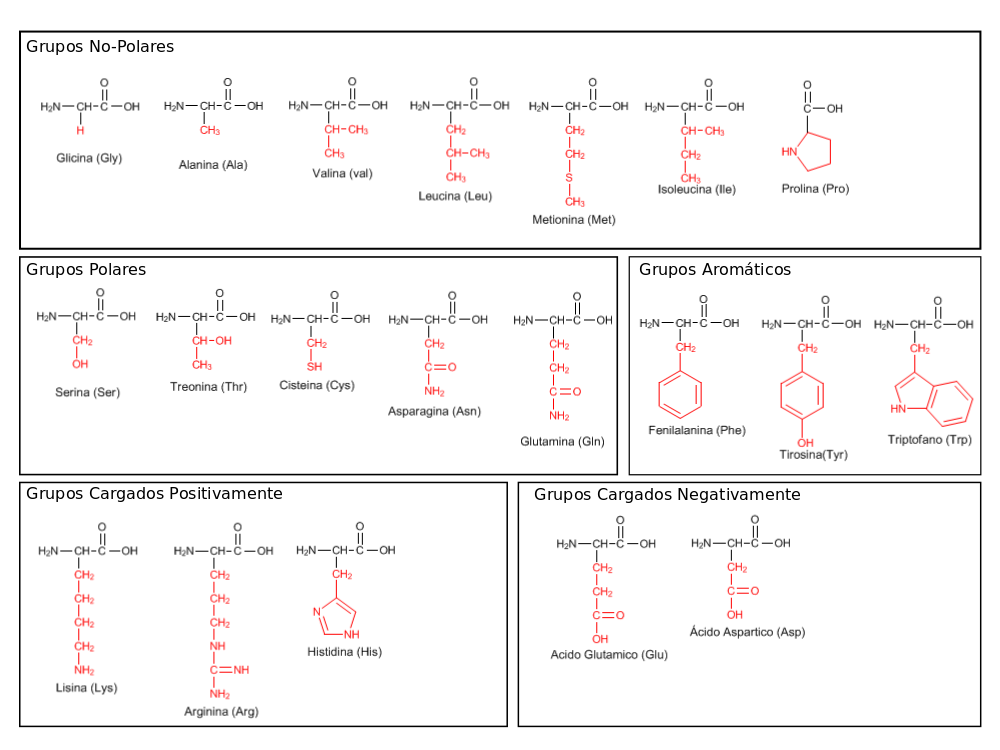
\includegraphics[width=1.3\textwidth]{Figure/aa2.png}
\end{figure}}
\only<4>{\begin{figure}
    \centering
    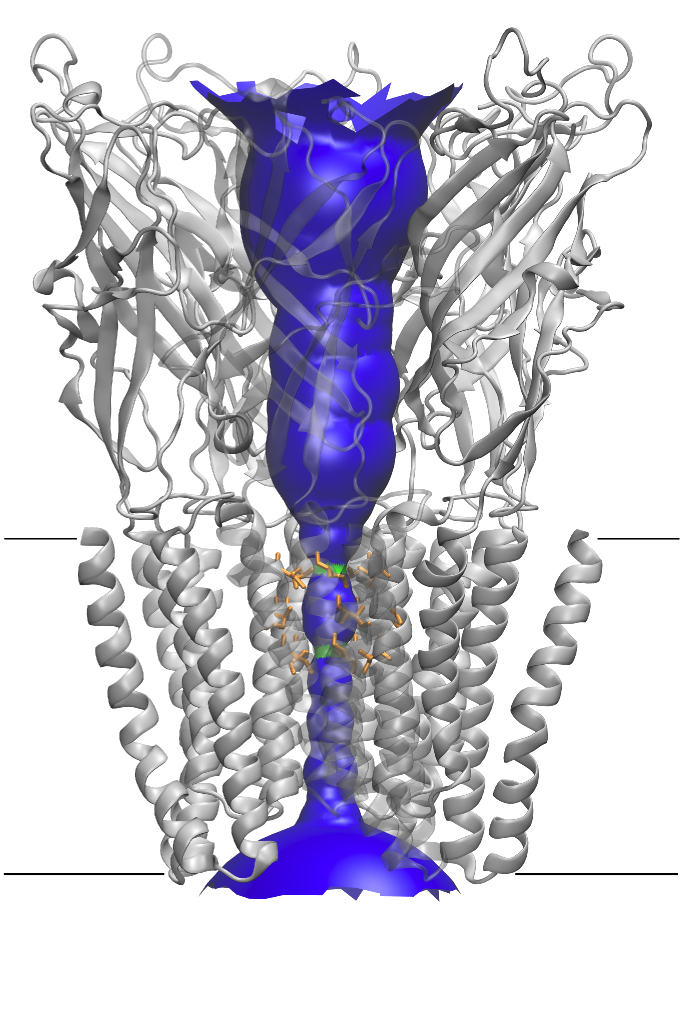
\includegraphics[width=0.9\textwidth]{Figure/GLIC.png}    
\end{figure}}
\end{minipage}
\end{frame}


% \begin{frame}[t]
% \justifying
% \begin{wrapfigure}{r}{0.5\textwidth}
% \Centering
% \only<1>{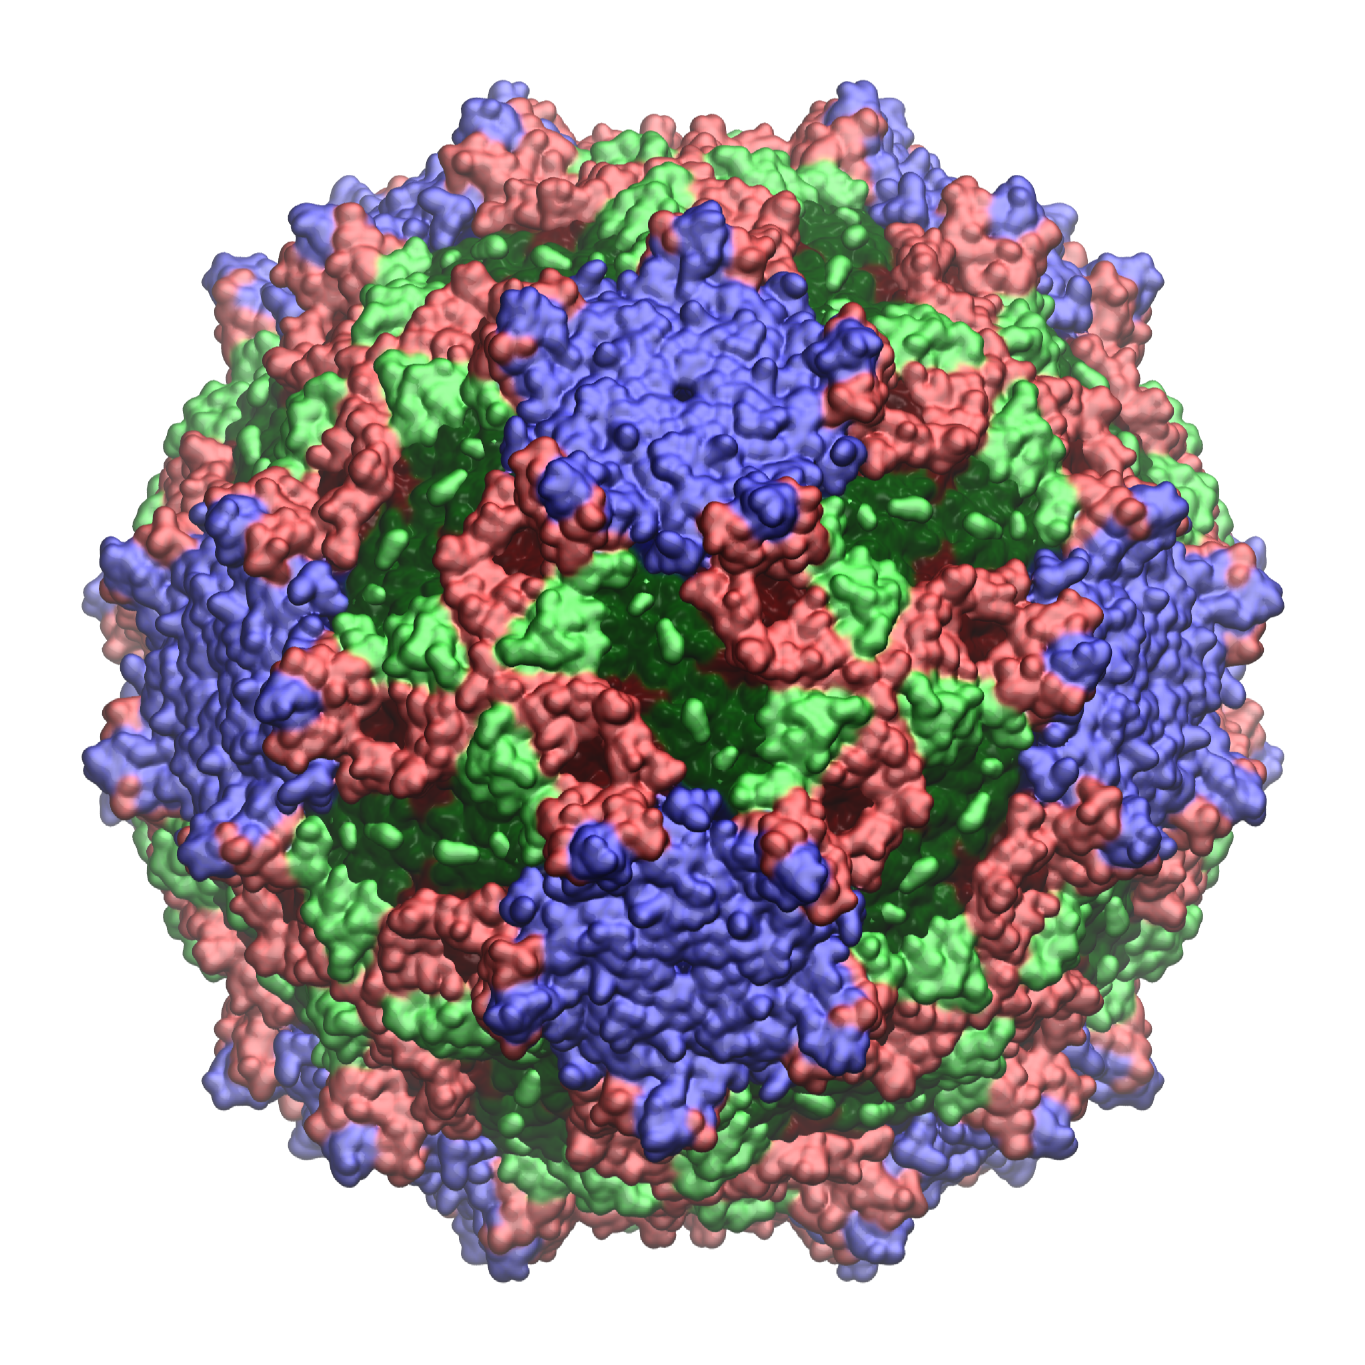
\includegraphics[width=0.5\textwidth]{Figure/TrV_Capsid.png}}
% \only<2>{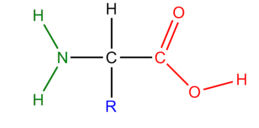
\includegraphics[width=0.3\textwidth]{Figure/aa.jpg} \\
% 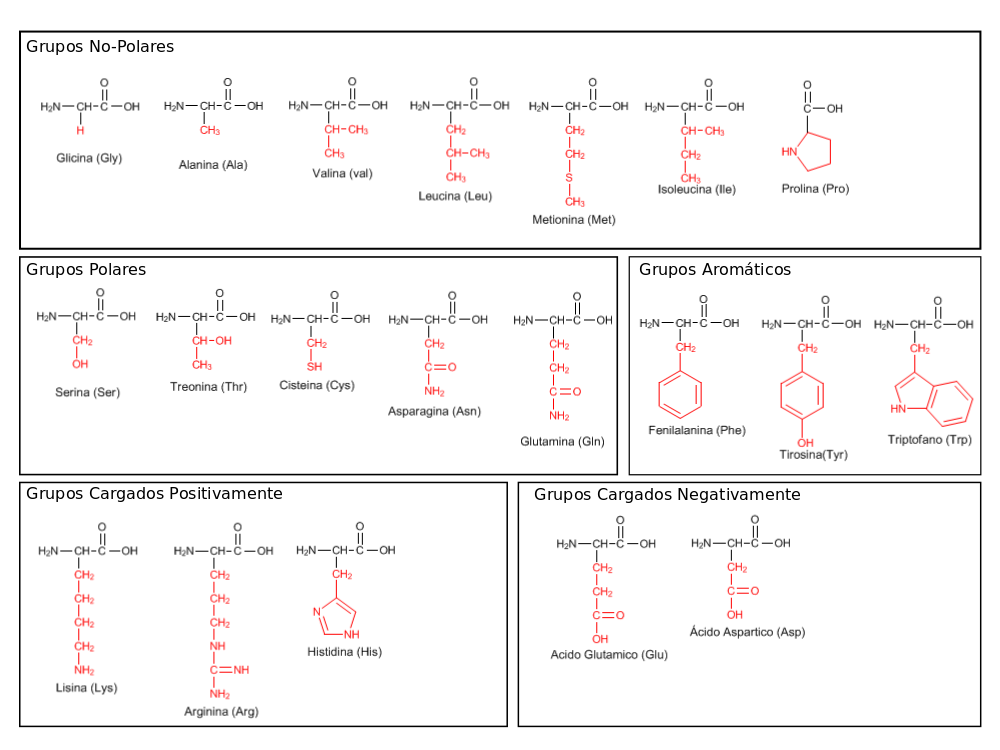
\includegraphics[width=0.5\textwidth]{Figure/aa2.png}}
% \only<3>{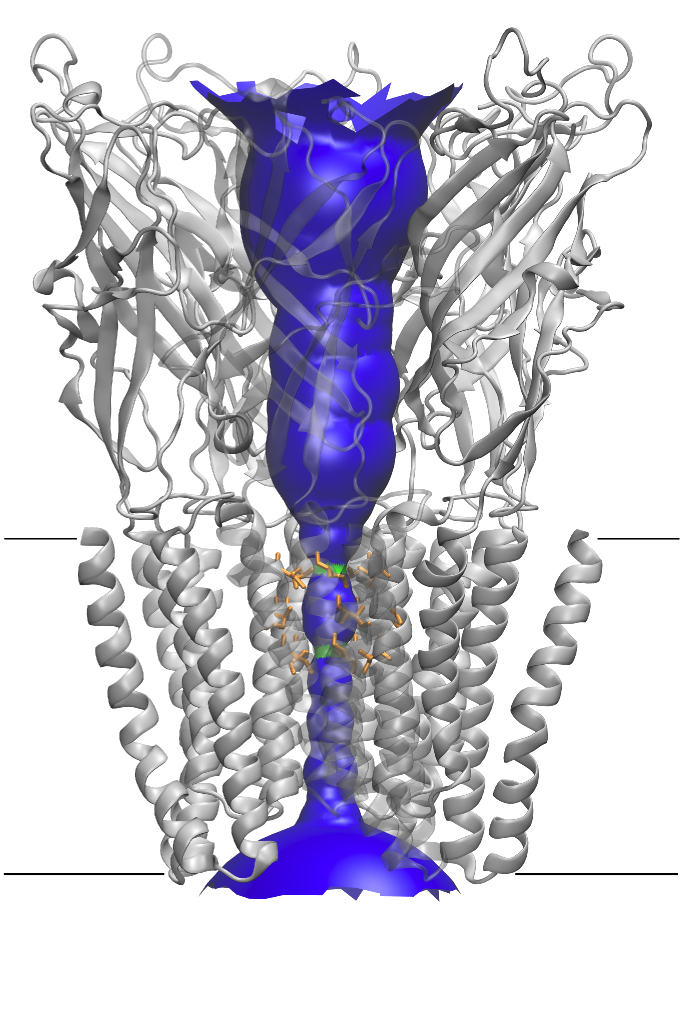
\includegraphics[width=0.5\textwidth]{Figure/GLIC.png}}
% \end{wrapfigure}
% $\bullet$ Las cápsides virales son estructuras proteicas cuya función consiste en proteger el material genético del virus y son las encargadas de interactuar con el medio y comenzar el proceso de infección. Sin embargo, este proceso no ha sido completamente explicado aún.
% \invisible<-1>{ \vspace{0.1cm}
% $\bullet$ Las proteínas son componentes químicos de las sustancias orgánicas. Estructuralmente son cadenas lineales cuyos monómeros son los aminoácidos. Los cuales están formados por un grupo amino ($-NH_2$ ), un grupo  ácido o carboxilo ($-COOH$) y un grupo (R) que varia en cada uno de los veinte aminoácidos que existen en la naturaleza.}
% \invisible<-2>{ \vspace{0.1cm}
% $\bullet$ Un grupo muy estudiado de proteínas, son las proteínas que interactúan con las membranas celulares, particularmente las canales iónicos. Estas proteínas presentan estructuras macromoleculares complejas cuya función es el transporte de ciertas moléculas entre el exterior y el interior de las células.}
% \end{frame}


\begin{frame}[t]
%\vspace{-1cm}
\justifying
Los virus icosaédricos, como los del género Picornavirales, poseen cápsides con gran simetría. Estas cápsides poseen varios ejes de simetría dobles, triples y quíntuples. Particularmente, se ha propuesto que la cavidad presente en el eje de simetría quíntuple podría ejercer un rol como canal de iones (\textit{Susana Kalko et al.}). Sin embargo, esta hipótesis no ha sido corroborada.

\only<1>{
\begin{figure}[ht]
\centering
\hspace*{\fill}
\begin{subfigure}[t]{.46\textwidth}
  \centering
  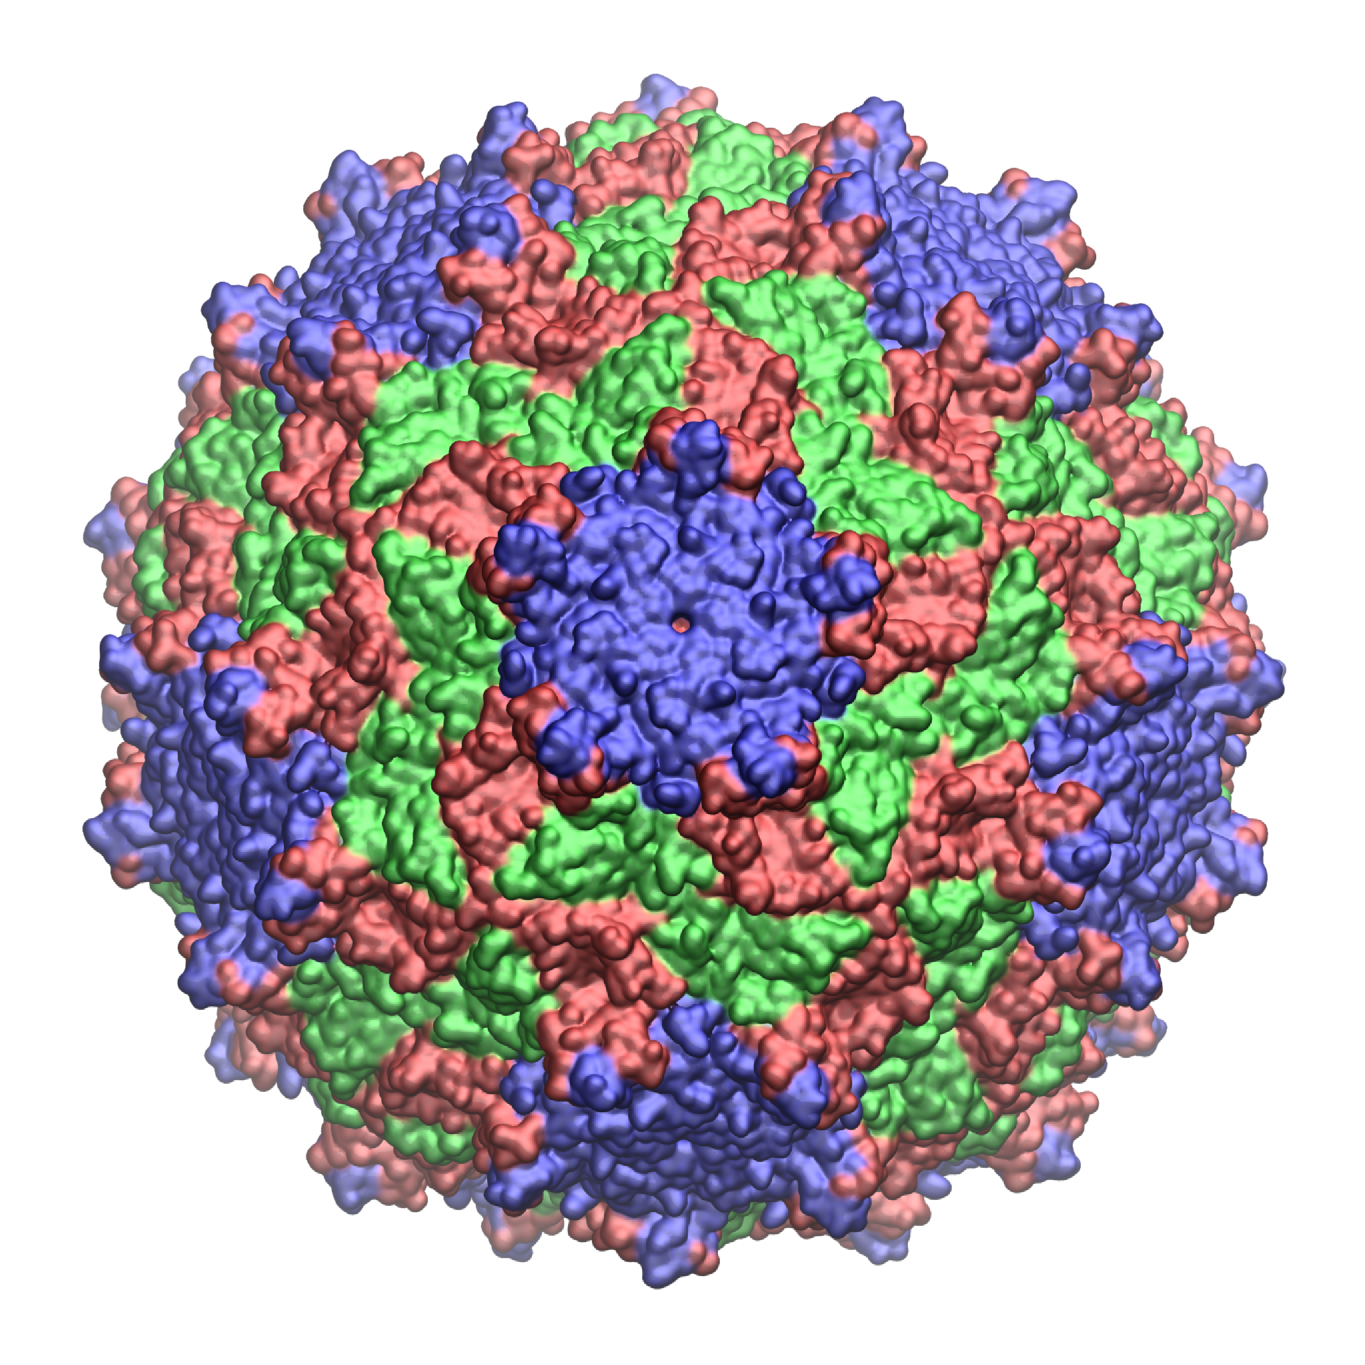
\includegraphics[width=1\textwidth]{Figure/TrV_Capsid_Ch4.png}
\end{subfigure}
\hspace*{\fill}
\begin{subfigure}[t]{.46\textwidth}
  \centering
  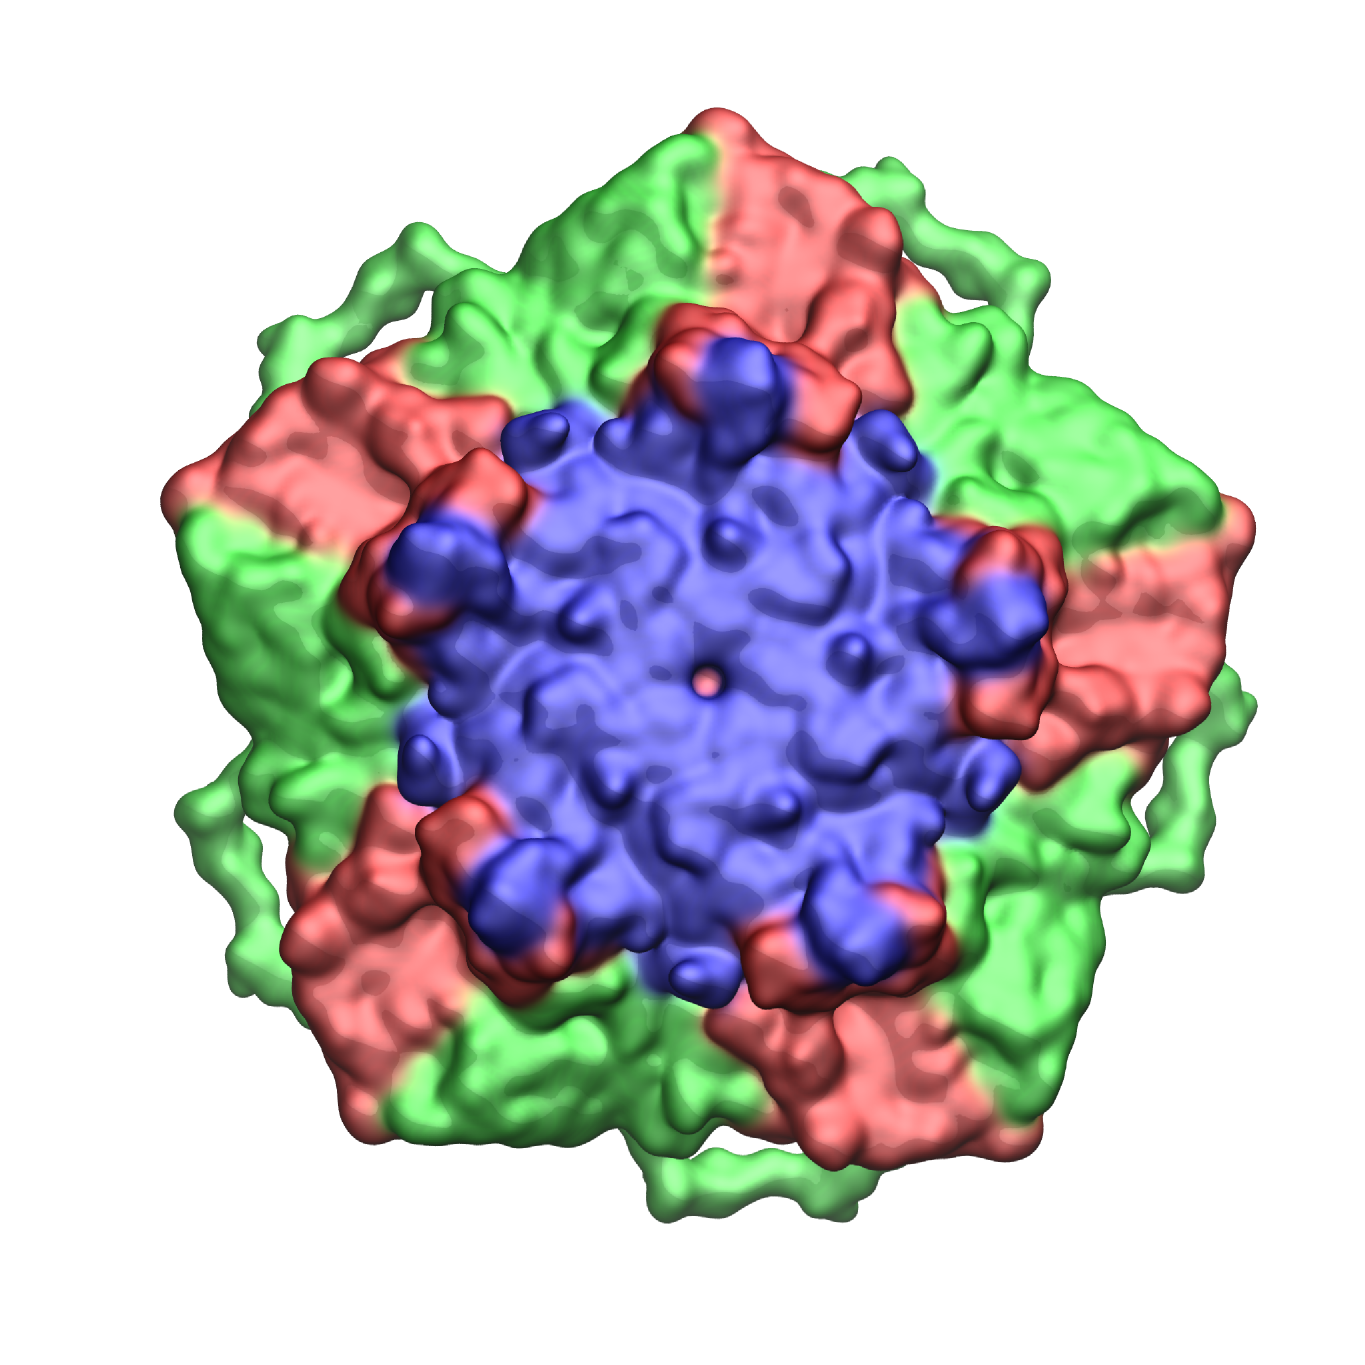
\includegraphics[width=1\textwidth]{Figure/TrV_Pentamer_Ch4.png}
  \end{subfigure}
\hspace*{\fill}
\end{figure}
}

\only<2>{
\centering
\begin{figure}[ht]
  \centering
  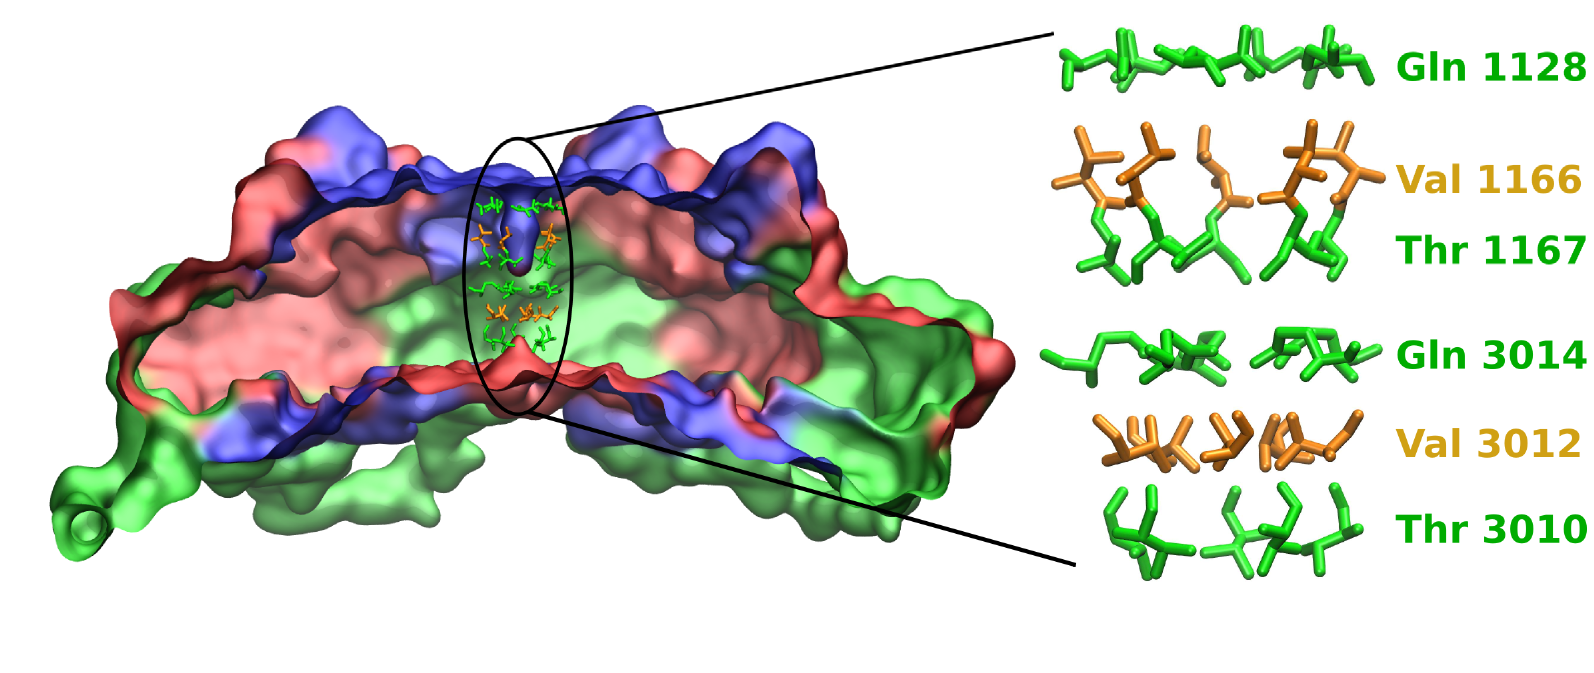
\includegraphics[width=1\textwidth]{Figure/TrV_Sideview_Pore.png}
\end{figure}
}

\end{frame}

%En que consiste el desensamblaje de un virus, que es lo que se sabe y que no.

%
% Objetivos
%

\subsection*{Objetivos}
\begin{frame}[t]{Objetivos}
\justifying
\begin{wrapfigure}{r}{0.4\textwidth}
\vspace{-0.5cm}
\Centering
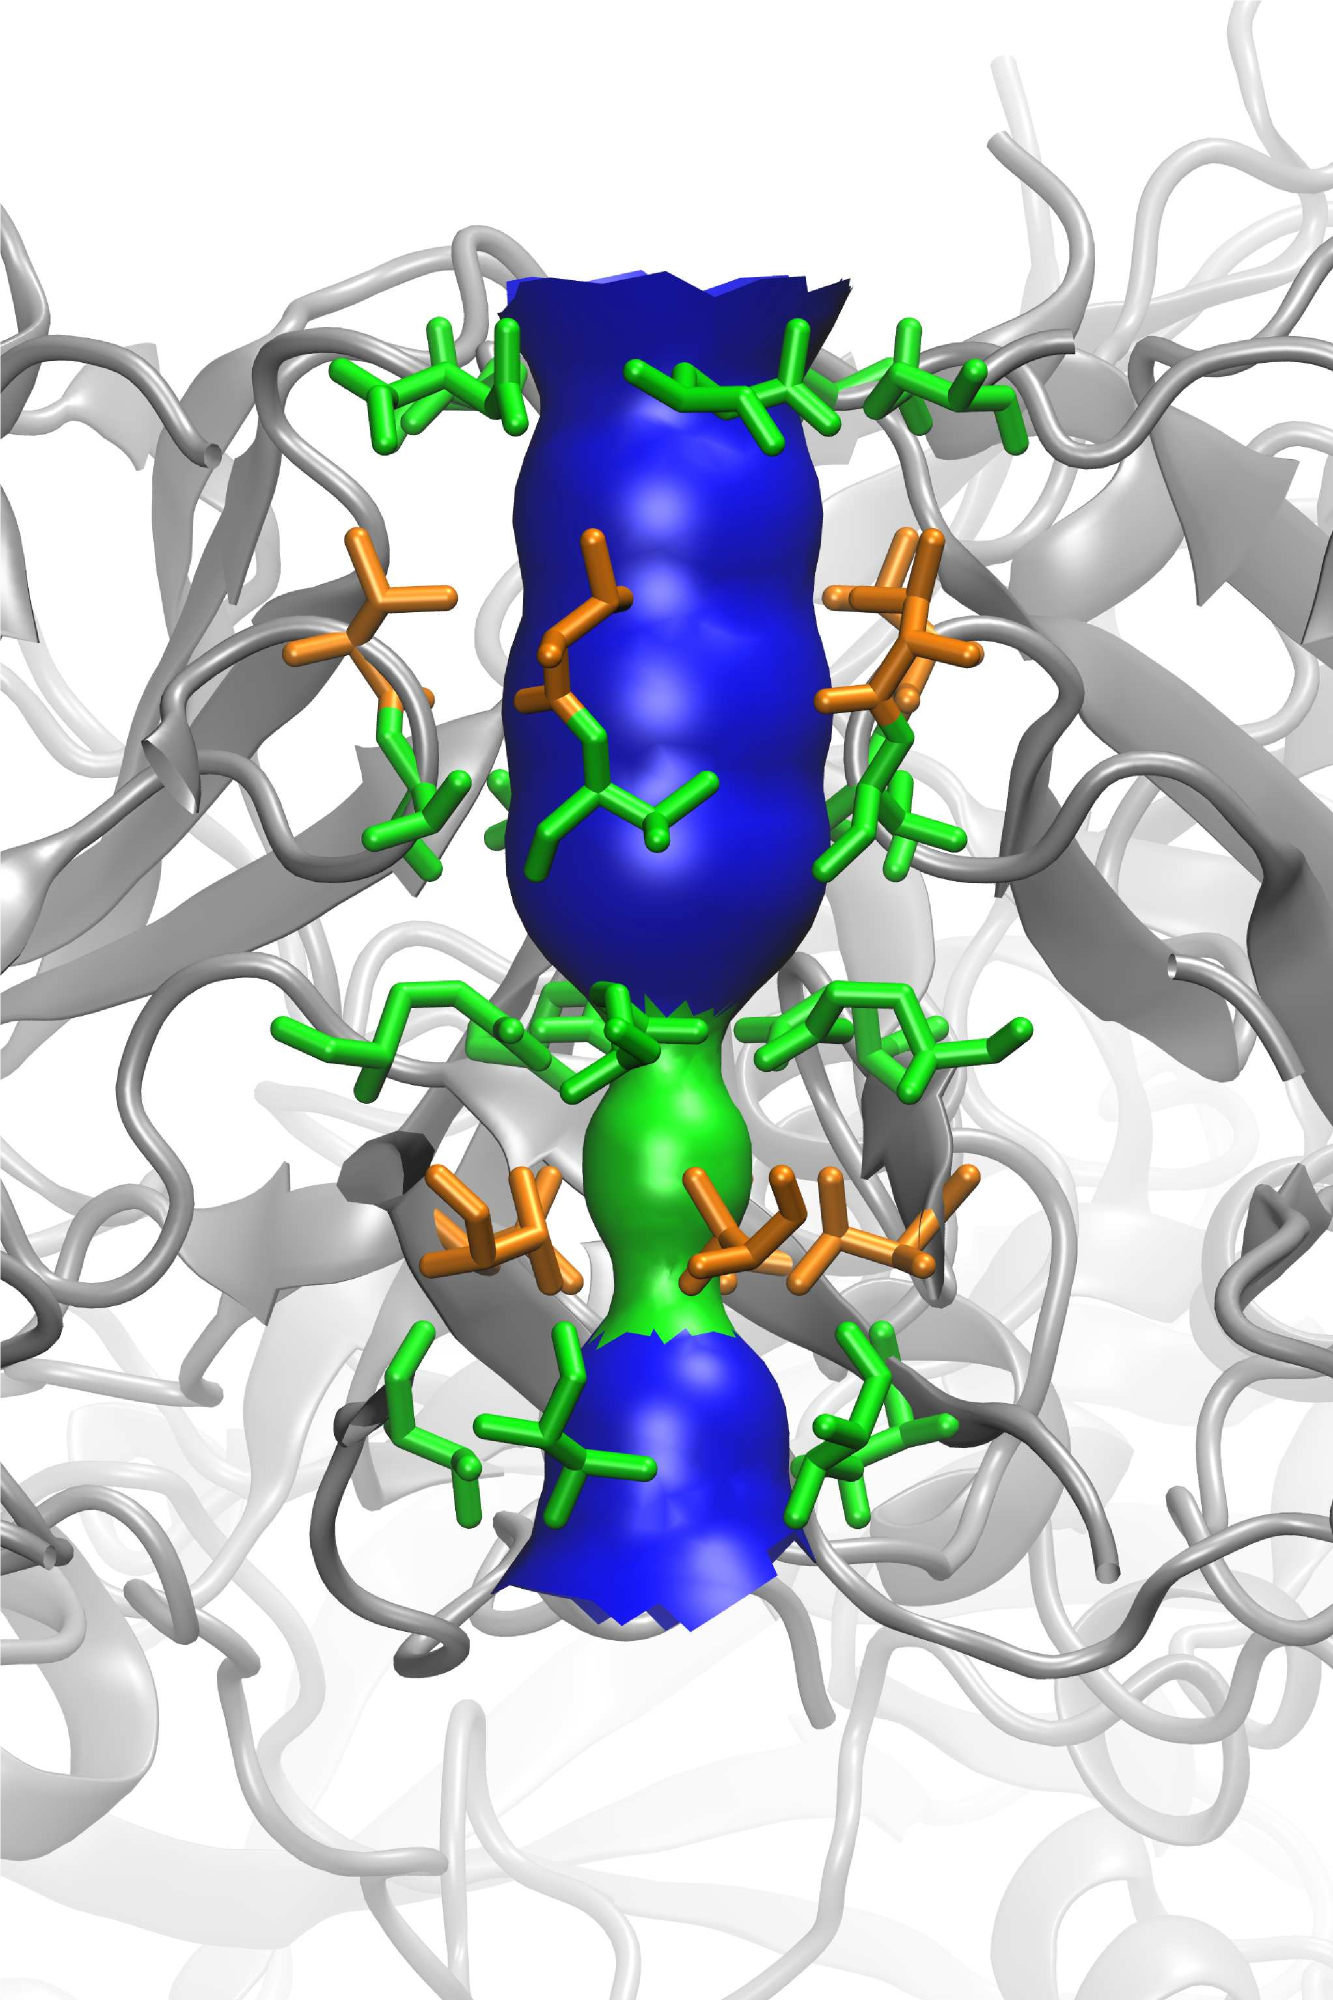
\includegraphics[width=0.35\textwidth]{Figure/TrV_Sideview_Pore_2.png}
\end{wrapfigure}

El objetivo de esta tesis es lograr determinar, a partir de técnicas computacionales, el rol de la cavidad presente en el eje de simetría quíntuple en el virus del Triatoma.
\begin{itemize}
\justifying
\item[$\bullet$] Determinar si el poro de TrV tiene función de canal.
\item[$\bullet$] Determinar si el poro posee algún mecanismo de regulación de su apertura.
\item[$\bullet$] Determinar que tipo de moléculas son capaces de atravesarlo.
\item[$\bullet$] Determinar similitudes y diferencias entre la estructura del eje quíntuple con la estructura de otros virus pertenecientes al género.
\end{itemize}

\end{frame}

% These three lines create an automatically generated table of contents.
\begin{frame}[t]
  \tableofcontents
\end{frame}

\AtBeginSection[]{        % Frame added before each section
  \frame<handout:0>{
    \tableofcontents[current]                   % Highlight current section/subsection
  }}

%
% Introducción
%

\section{Introducción}
\subsection{Virus del Triatoma}
\begin{frame}{Virus del Triatoma - TrV}
    \begin{center}
    \large{
    \textit{Picornavirales} $\rightarrow$ \textit{Dicistrovirus} $\rightarrow$ 
    \tikzmarkin<2->[set fill color=green!10, set border color=green]{f1}  
    \tikz[remember picture,baseline,inner sep=1ex]\node[anchor=base](n1){Triatoma Virus.}; \tikzmarkend{f1}
    }
    \end{center}
    \vspace{1cm}
    
    \onslide<2->{
    $\bullet$  \tikzmarkin<2->[set fill color=green!10, set border color=green]{f2} \tikz[remember picture,baseline,inner sep=0]\node[anchor=base](n2){Patógeno Natural}; \tikzmarkend{f2}
    del \textit{Triatoma Infestans}, insecto mejor conocido en América Latina como 
    \tikzmarkin<3->[set fill color=red!10, set border color=red]{f3} 
    \tikz[remember picture,baseline,inner sep=1ex]\node[anchor=base](n3){Vinchuca.};
    \tikzmarkend{f3}\\
    }
    \vspace{0.5cm}
    
    \onslide<3->{
    $\bullet$ Principal 
    \tikzmarkin<3->[set fill color=red!10, set border color=red]{f4} 
    \tikz[remember picture,baseline,inner sep=1ex]\node[anchor=base](n4){vector};
    \tikzmarkend{f4} de la \textit{Trypanosomiasis Americana} o Mal de Chagas.\\
    }

\begin{tikzpicture}[remember picture,overlay]
\draw<2->[thick,green,->] (n1) -- (n2);
\end{tikzpicture}
\begin{tikzpicture}[remember picture,overlay]
\draw<3->[thick,red,->] (n3) -- (n4);
\end{tikzpicture}
    
\end{frame}

\subsection{Dinámica Molecular}
\begin{frame}[t]{Dinámica Molecular}

Integrador de Leap-Frog:
\begin{align*}
&x(t+\Delta t) = x(t) + v(t+\frac{1}{2}\Delta t){\Delta t} \nonumber \\
&v(t+\frac{1}{2}\Delta t) = v(t-\frac{1}{2}\Delta t) + a\Delta t
\end{align*}

\invisible<-1>{
Campo de Fuerzas:
\begin{multline*}
V = \tikzmarkin<3->[set fill color=green!10, set border color=green!30!black!80]{cc}(0,-0.4)(0,0.4) \sum\limits_{enlaces} \frac{k_{b,i}}{2} (l_i-l_{i0})^2 \tikzmarkend{cc}
+ \tikzmarkin<3->[set fill color=green!10, set border color=green!30!black!80]{dd}(0,-0.4)(0,0.4) \sum\limits_{angulos} \frac{k_{\theta,i}}{2} (\theta_i-\theta_{i,0})^2 \tikzmarkend{dd}
+ \tikzmarkin<3->[set fill color=green!10, set border color=green!30!black!80]{ee}(0,-0.4)(0,0.4) \sum\limits_{torsiones} \frac{\nu_n}{2} (1+cos(n\omega-\gamma)) \tikzmarkend{ee} \\
+ \sum\limits_{i=1} \sum\limits_{j=i+1} (
\tikzmarkin<3->[set fill color=red!10, set border color=red]{aa}(0,-0.4)(0,0.4) 4\epsilon[(\frac{\sigma_{ij}}{r_{ij}})^{12}-(\frac{\sigma_{ij}}{r_{ij}})^6] \tikzmarkend{aa}
+ \tikzmarkin<3->[set fill color=blue!10, set border color=blue]{bb}(0,-0.4)(0,0.4) \frac{q_iq_j}{4\pi\epsilon_0r_{ij}} \tikzmarkend{bb}
)
\end{multline*}
}

\begin{minipage}{0.4\textwidth}
\invisible<-1>{
\vspace{-0.5cm}
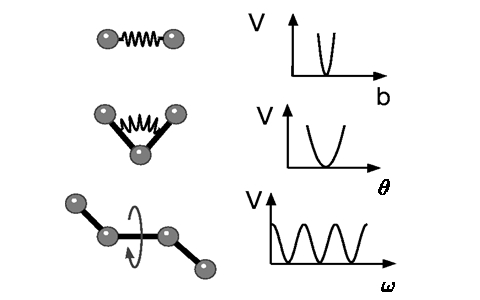
\includegraphics[width=\textwidth]{Figure/ff.jpg}
}
\end{minipage}
\begin{minipage}{0.59\textwidth}
\invisible<-2>{
  \vspace{-0.5cm}
  \begin{center}
  \begin{tabular}{cl}
  {\color{green!30!black!80} Potencial enlazante: enlaces} \\
  {\color{green!30!black!80} Potencial enlazante: ángulos} \\
  {\color{green!30!black!80} Potencial enlazante: torsiones} \\
  {\color{red} Potencial Coulombiano} \\ 
  {\color{blue} Potencial de Lennard-Jones}
  \end{tabular}
  \end{center}
}
\end{minipage}

\end{frame}

\subsection{Campos de Fuerza}
\begin{frame}[t]{Campos de Fuerza}
\justifying


\begin{wrapfigure}{r}{0.7\textwidth}
\begin{figure}[ht]
\centering
\hspace*{\fill}
\begin{subfigure}[t]{.32\textwidth}
  \vspace{-1cm}
  \centering
  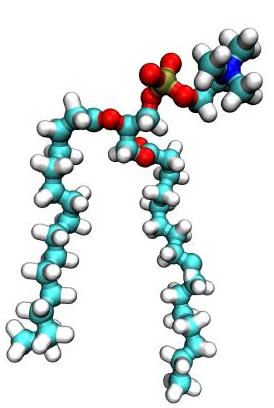
\includegraphics[width=0.8\textwidth]{Figure/FF-AA.png}
\end{subfigure}
\onslide<2->{
\hspace*{\fill}
\begin{subfigure}[t]{.32\textwidth}
  \vspace{-1cm}
  \centering
  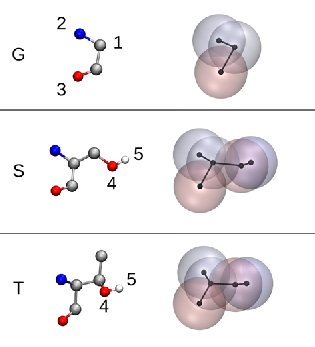
\includegraphics[width=0.8\textwidth]{Figure/FF-CG.png}
\end{subfigure}
}
\hspace*{\fill}
\onslide<3->{
\begin{subfigure}[t]{.5\textwidth}
  \vspace{-0.1cm}
  \centering
  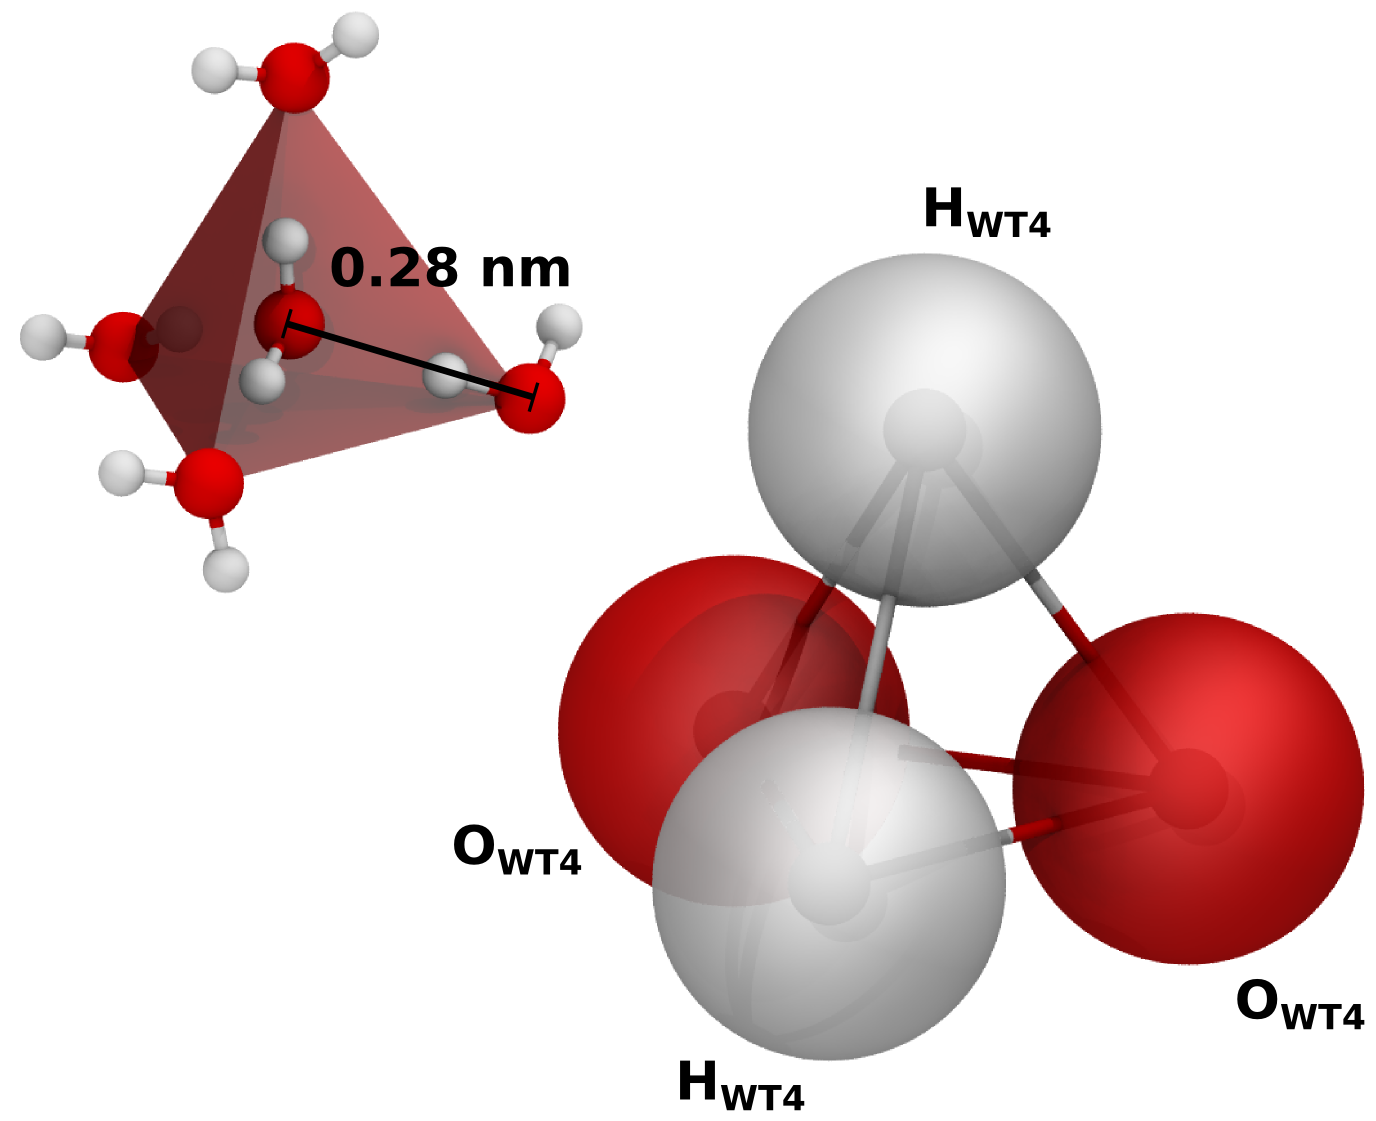
\includegraphics[width=0.8\textwidth]{Figure/FF-wt4.png}
\end{subfigure}
}
\hspace*{\fill}
\end{figure}
\end{wrapfigure}


\textbf{Atomísticos}
\begin{enumerate}
    \item \tikzmarkin<4->[set fill color=red!10, set border color=red]{a} GROMOS \tikzmarkend{a}
    \item AMBER
    \item CHARMM
    \item OPLS
\end{enumerate}
\vspace{0.5cm}

\onslide<2->{
\textbf{Grano Grueso}
\begin{enumerate}
    \item \tikzmarkin<4->[set fill color=red!10, set border color=red]{b} Sirah \tikzmarkend{b}
    \item Martini
\end{enumerate}
\vspace{0.5cm}
}

\onslide<3->{
\textbf{Modelos de Agua}
\begin{enumerate}
    \item \tikzmarkin<4->[set fill color=red!10, set border color=red]{c} SPC \tikzmarkend{c}
    \item SPC/e
    \item TIP3P
    \item \tikzmarkin<4->[set fill color=red!10, set border color=red]{d} WT4 y WLS \tikzmarkend{d}
\end{enumerate}
}

\end{frame}

\begin{frame}[t]{Dinámica Molecular}
\onslide<1->\centering \large{\textbf{Gromacs}} \\
\only<1>{
\includegraphics[width=0.6\textwidth]{Figure/GROMACS.png}}

\hspace{-1cm}
\begin{minipage}[t]{0.42\textwidth}
\begin{itemize}
    \setlength\itemsep{1em}
    \item<2-> Caja de simulación: \textbf{Dodecaédrica}
    \item<3-> Condiciones de borde Periódic.
    \item<4-> Termostáto:
    \tikzmarkin<4>[set fill color=red!10, set border color=red]{eq11}
    Berendsen \tikzmarkend{eq11} o
    \tikzmarkin<4>[set fill color=blue!10, set border color=blue]{eq22}
    v-rescale. \tikzmarkend{eq22} 
    \item<4-> Barostáto:
    \tikzmarkin<4>[set fill color=green!10, set border color=green]{eq33}
    Berendsen \tikzmarkend{eq33} o
    \tikzmarkin<4>[set fill color=violet!10, set border color=violet]{eq44}
    Parrinello-Rahman. \tikzmarkend{eq44}
\end{itemize}
\end{minipage}
\hspace{1cm}
\begin{minipage}[t]{0.55\textwidth}
\vspace{1cm}
\only<2>{
\begin{figure}[ht]
  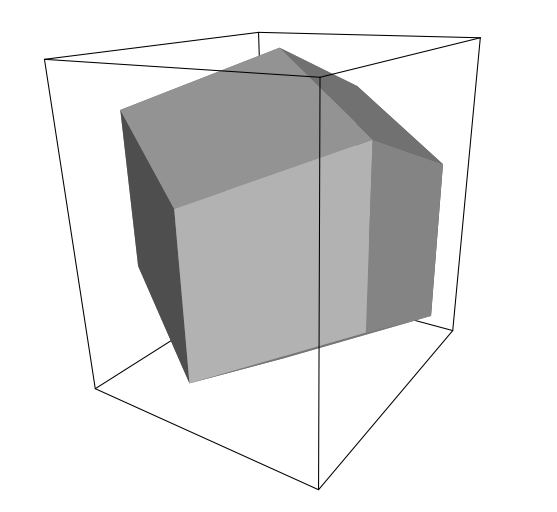
\includegraphics[width=0.8\textwidth]{Figure/box.png}
\end{figure}}
\only<3>{
\begin{figure}[ht]
  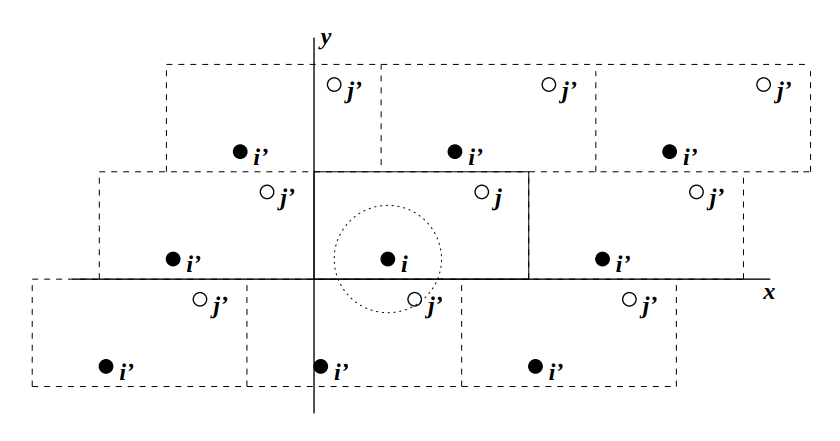
\includegraphics[width=0.8\textwidth]{Figure/pbc.png}
\end{figure}}
\only<4>{
\begin{equation*}
\tikzmarkin<4>[set fill color=red!10, set border color=red]{eq1}(0,-0.4)(0,0.6)
\frac{dT(t)}{dt}=\frac{1}{\tau}(T_{ba\tilde{n}o}-T(t))
\tikzmarkend{eq1}
\end{equation*}
\begin{equation*}
\tikzmarkin<4>[set fill color=blue!10, set border color=blue]{eq2}(0,-0.4)(0,0.6)
dK=\frac{dt}{\tau}(K_{ba\tilde{n}o}-K)+2\sqrt{\frac{KK_{ba\tilde{n}o}}{N_l}\frac{dW}{\sqrt{\tau}}}
\tikzmarkend{eq2}
\end{equation*}
\begin{equation*}
\tikzmarkin<4>[set fill color=green!10, set border color=green]{eq3}(0,-0.4)(0,0.6)
\frac{dP(t)}{dt}=\frac{1}{\tau}(P_{ba\tilde{n}o}-P(t))
\tikzmarkend{eq3}
\end{equation*}
\begin{equation*}
\tikzmarkin<4>[set fill color=violet!10, set border color=violet]{eq4}(0,-0.4)(0,0.6)
\frac{d\bm{b}^2}{dt^2}=V\bm{W}^{-1}\bm{b}'^{-1}(P-P_0)
\tikzmarkend{eq4}
\end{equation*}
}
\end{minipage}
\end{frame}

%
% Poro en el eje quíntuple de TrV
%

\section{Puerta Hidrofóbica}
\subsection{Poro en el Eje Quíntuple de TrV}
\begin{frame}[t]{Poro en el Eje Quíntuple de TrV}
\hspace{-0.7cm}
\begin{minipage}{0.4\textwidth}
\justifying
\begin{enumerate}[$\bullet$]
\item Estudio de la hidratación.
\item Dinámica Molecular a multiescala.
\item Proteína a nivel de detalle atómico.
\item Aguas periféricas a nivel de grano-grueso (Coarse-Grain).
\end{enumerate}
\end{minipage}
\hfill
\begin{minipage}{0.59\textwidth}
\onslide<2->{
\textbf{Protocolo}
\begin{itemize}
    \item Minimización de Energia: Steep Descent o Conjugate Gracients.
    \item Restricción de Posiciones: proteína fijas y aguas libres.
    \item Termalización: 1 ns de 100 K a 310 K.
    \item Simulaciones de Producción: hasta 100 ns.
\end{itemize}
}
\end{minipage}
\vspace{0.5cm}
\begin{center}
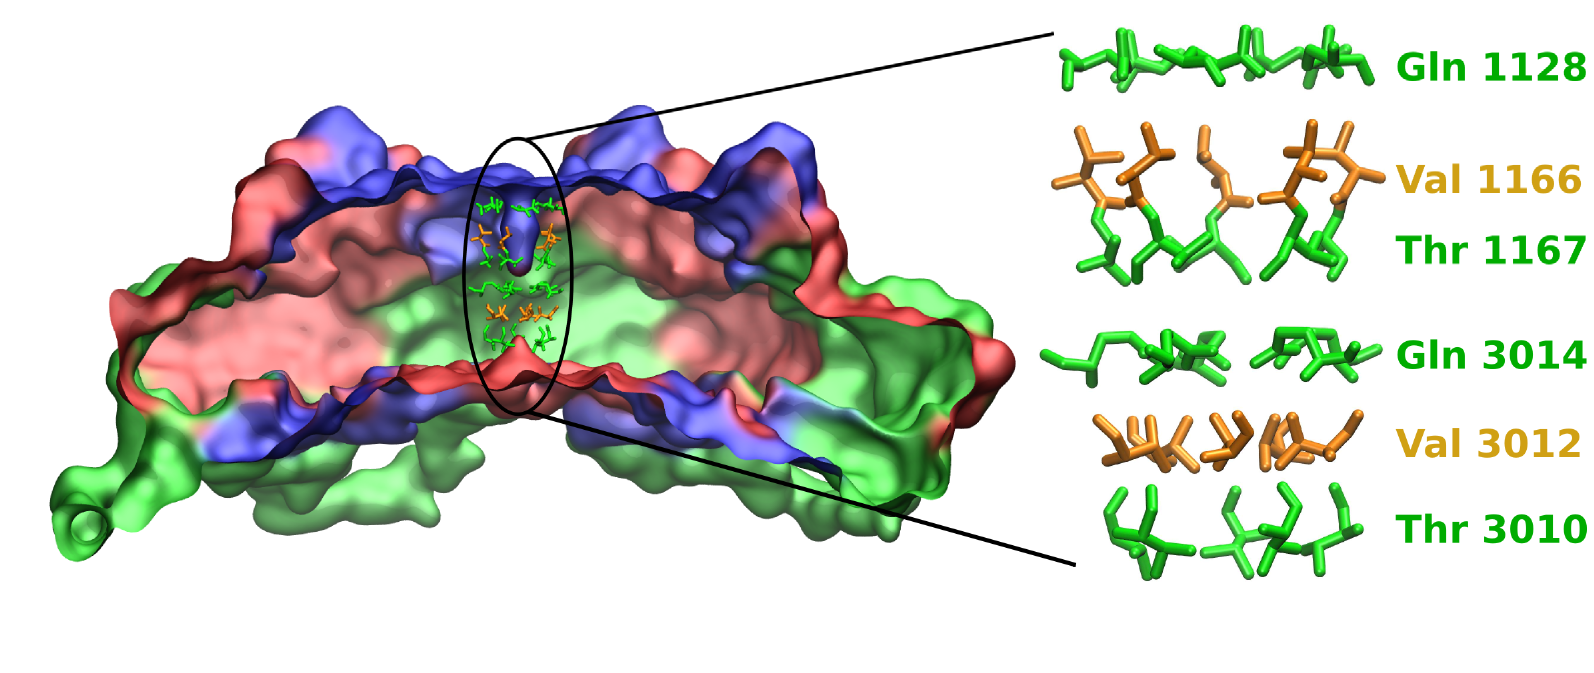
\includegraphics[width=0.8\textwidth]{Figure/TrV_Sideview_Pore.png}
    
\end{center}
\end{frame}

\subsection{Sistema a Simular}
\begin{frame}[t]{Sistema a Simular}

\begin{figure}[ht]
\vspace{-0.4cm}
\centering
\hspace*{\fill}
\begin{subfigure}[t]{.46\textwidth}
  \centering
  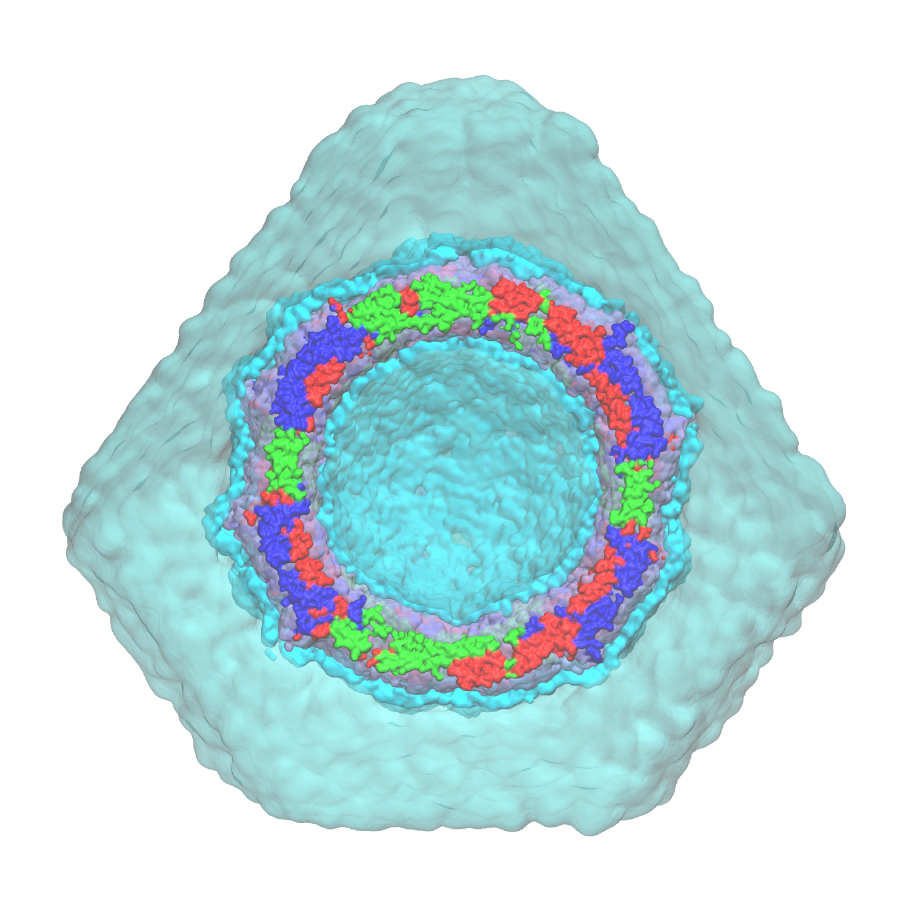
\includegraphics[width=1\textwidth]{Figure/TrV_Capsid_WaterBox.png}
  \vspace{-0.5cm}
  \caption*{hellou}
  \label{fig:trv_capsid_waterbox}
\end{subfigure}
\hspace*{\fill}
\begin{subfigure}[t]{.46\textwidth}
  \centering
  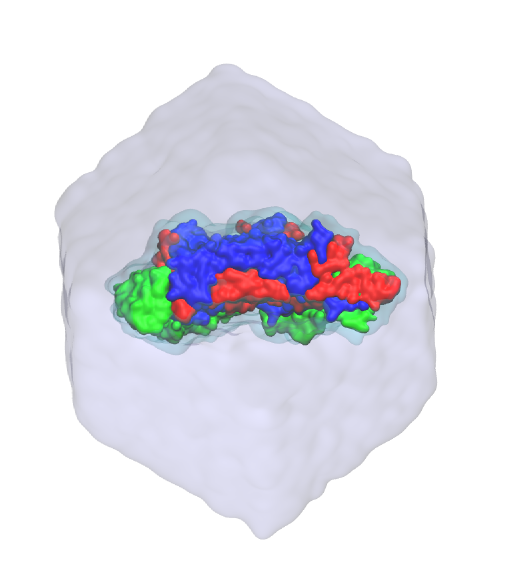
\includegraphics[width=1\textwidth]{Figure/TrV_Pentamer_WaterBox.png}
  \caption*{}
  \label{fig:trv_pentamer_waterbox}
\end{subfigure}
\hspace*{\fill}
%\vspace{-10mm}
\caption*{ Corte transversal del sistema de simulación, (a) cápside completa y (b) pentámero aislado. En azul, verde y rojo las superficies de las proteínas virales VP1, 2 y 3. Seguido de las capas de solvente SPC, WT4 y WLS representadas como superficies transparentes.}%
\end{figure}
\end{frame}

\subsection{Resultados - TrV Wild-Type}
\begin{frame}[t]{Resultados - TrV Wild-Type}
\begin{figure}[ht]
  \centering
    \vspace{-0.25cm}
  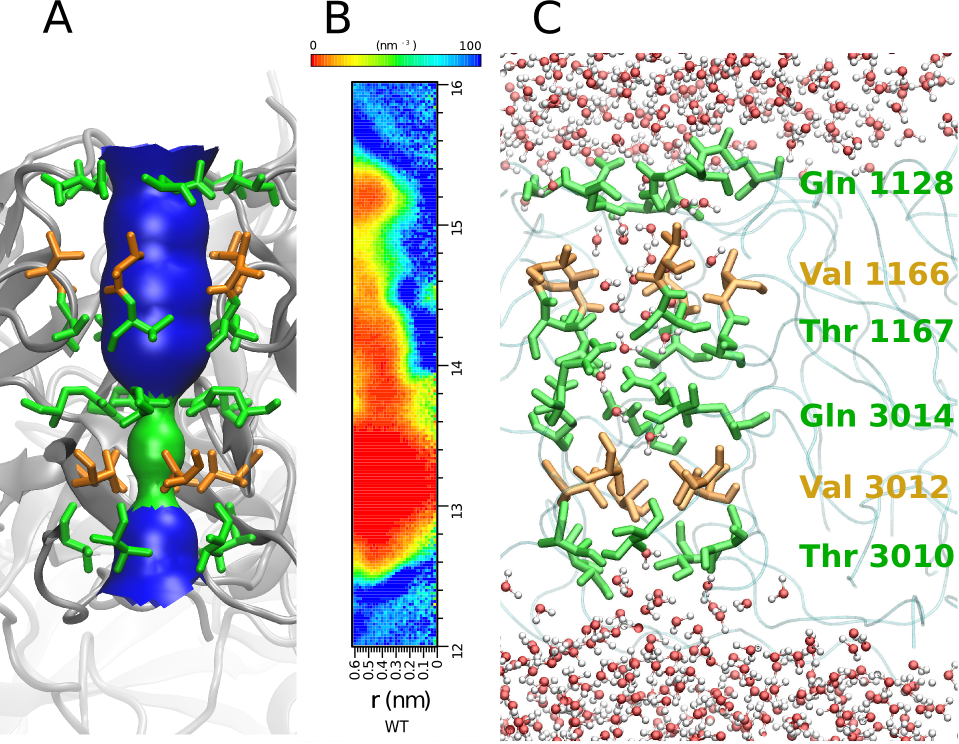
\includegraphics[height=6.3cm,keepaspectratio]{Figure/TrV_WT_Dens.png}
\caption*{ (A) Radio del poro. (B) Mapa de densidad de moléculas de agua. \\ (C) Vista lateral del poro de TrV.} %
\end{figure}
\end{frame}

\subsection{Resultados - TrV Mutación Valina por Serina}
\begin{frame}[t]{Resultados - TrV Mutación Valina por Serina}

\begin{figure}[ht]
  \centering
  \vspace{-0.25cm}
  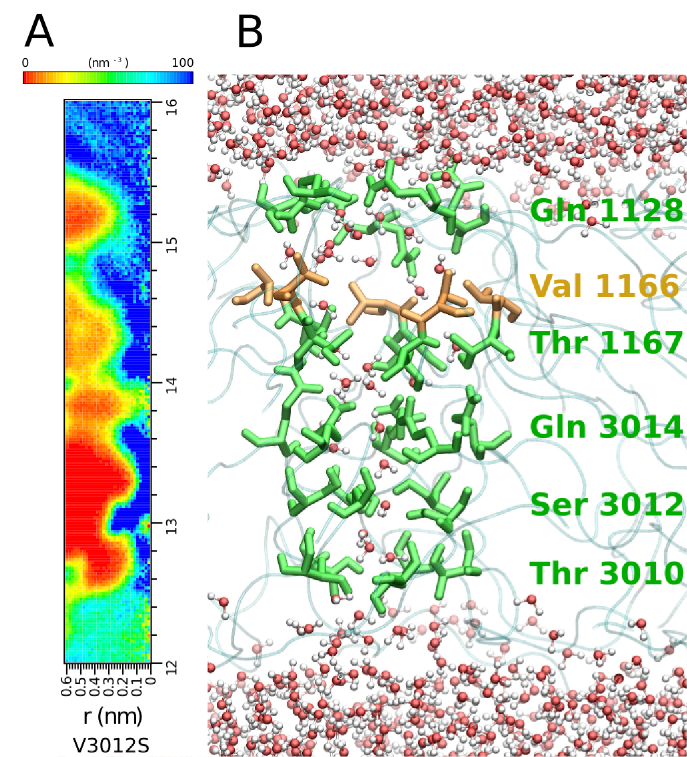
\includegraphics[height=6.3cm,keepaspectratio]{Figure/TrV_VS_Dens.png}
\caption*{ (A) Mapa de densidad de moléculas de agua. (B) Vista lateral del poro de TrV mutado.}%
\end{figure}

\end{frame}

\subsection{Conclusión I}
\begin{frame}{Conclusión I}
\begin{itemize}
    \item Se observa la existencia de un poro en el eje quíntuple de TrV capaz de comunicar el medio interior del virus con su exterior.\vfill
    \item Se observa la presencia de un posible medio de regulación del poro a través de una puerta hidrofóbica ubicada a la altura de las Valinas 3012.\vfill
    \item Estas características han sido observadas anteriormente en membranas celulares pero no así en cápsides virales.
\end{itemize}
\end{frame}

%
% Apertura de la Puerta
%

\section{Apertura de la Puerta}
\subsection{Densidad Electrónica Desconocida}
\begin{frame}{Mapa de Densidad Electrónica}
\centering
\begin{tikzpicture}
\node[anchor=south west,inner sep=0] at (0,0)
    {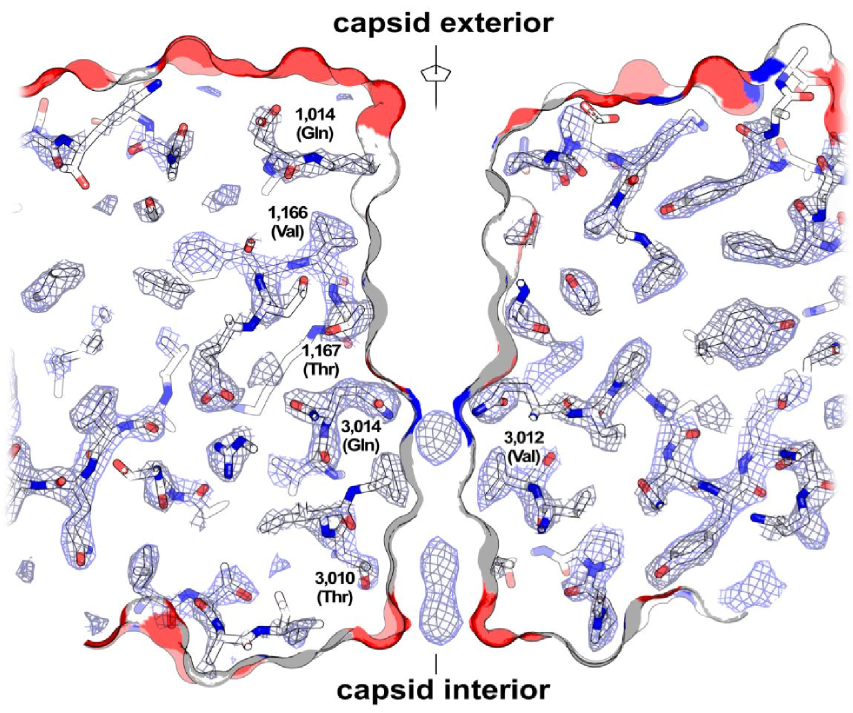
\includegraphics[height=6.5cm,keepaspectratio]{Figure/TrV_edens.png}};
    \draw<2>[red,ultra thick,rounded corners] (3.5,2.0) rectangle (4.5,3.0);
\end{tikzpicture} \\
\centering Mapa de densidad electrónica de TrV \\(Material Suplementario \textit{G. Squires et al 2013}).
\end{frame}

\subsection{Potencial de Fuerza Media}
\begin{frame}[t]{Perfil de Energía Libre en el poro de TrV}
La energía libre de Helmholtz viene dada por la expresión:
\begin{minipage}{0.4\textwidth}
\begin{equation*}
A = - k_B T ln Q
\end{equation*}
\end{minipage}
\onslide<2->{
\begin{minipage}{0.4\textwidth}
\begin{equation*}
A = k_B T ln(\iint d\bm{p}^N d\bm{r}^N 
\tikzmarkin<3->[set fill color=red!10, set border color=red]{pmf1}(0,-0.2)(0,0.6)
e^{\frac{E(\bm{p}^N,\bm{r}^N)}{k_B T}}
\tikzmarkend{pmf1}
\rho(\bm{p}^N,\bm{r}^N)
\end{equation*}
\end{minipage}
}
\vspace{0.2cm}

\begin{columns}
\column{0.5\textwidth}
\onslide<4->{

\centering
\large
\tikzmarkin<4->[set fill color=green!10, set border color=green]{pmf2}(1,-0.5)(0,0.5)
{Potencial de Fuerza Media\\ o\\ \textbf{PMF}\\
$+$\\
Umbrella Sampling}
\tikzmarkend{pmf2}
\vspace{1cm}
}
\column{0.5\textwidth}
\onslide<5->{
\begin{figure}[ht]
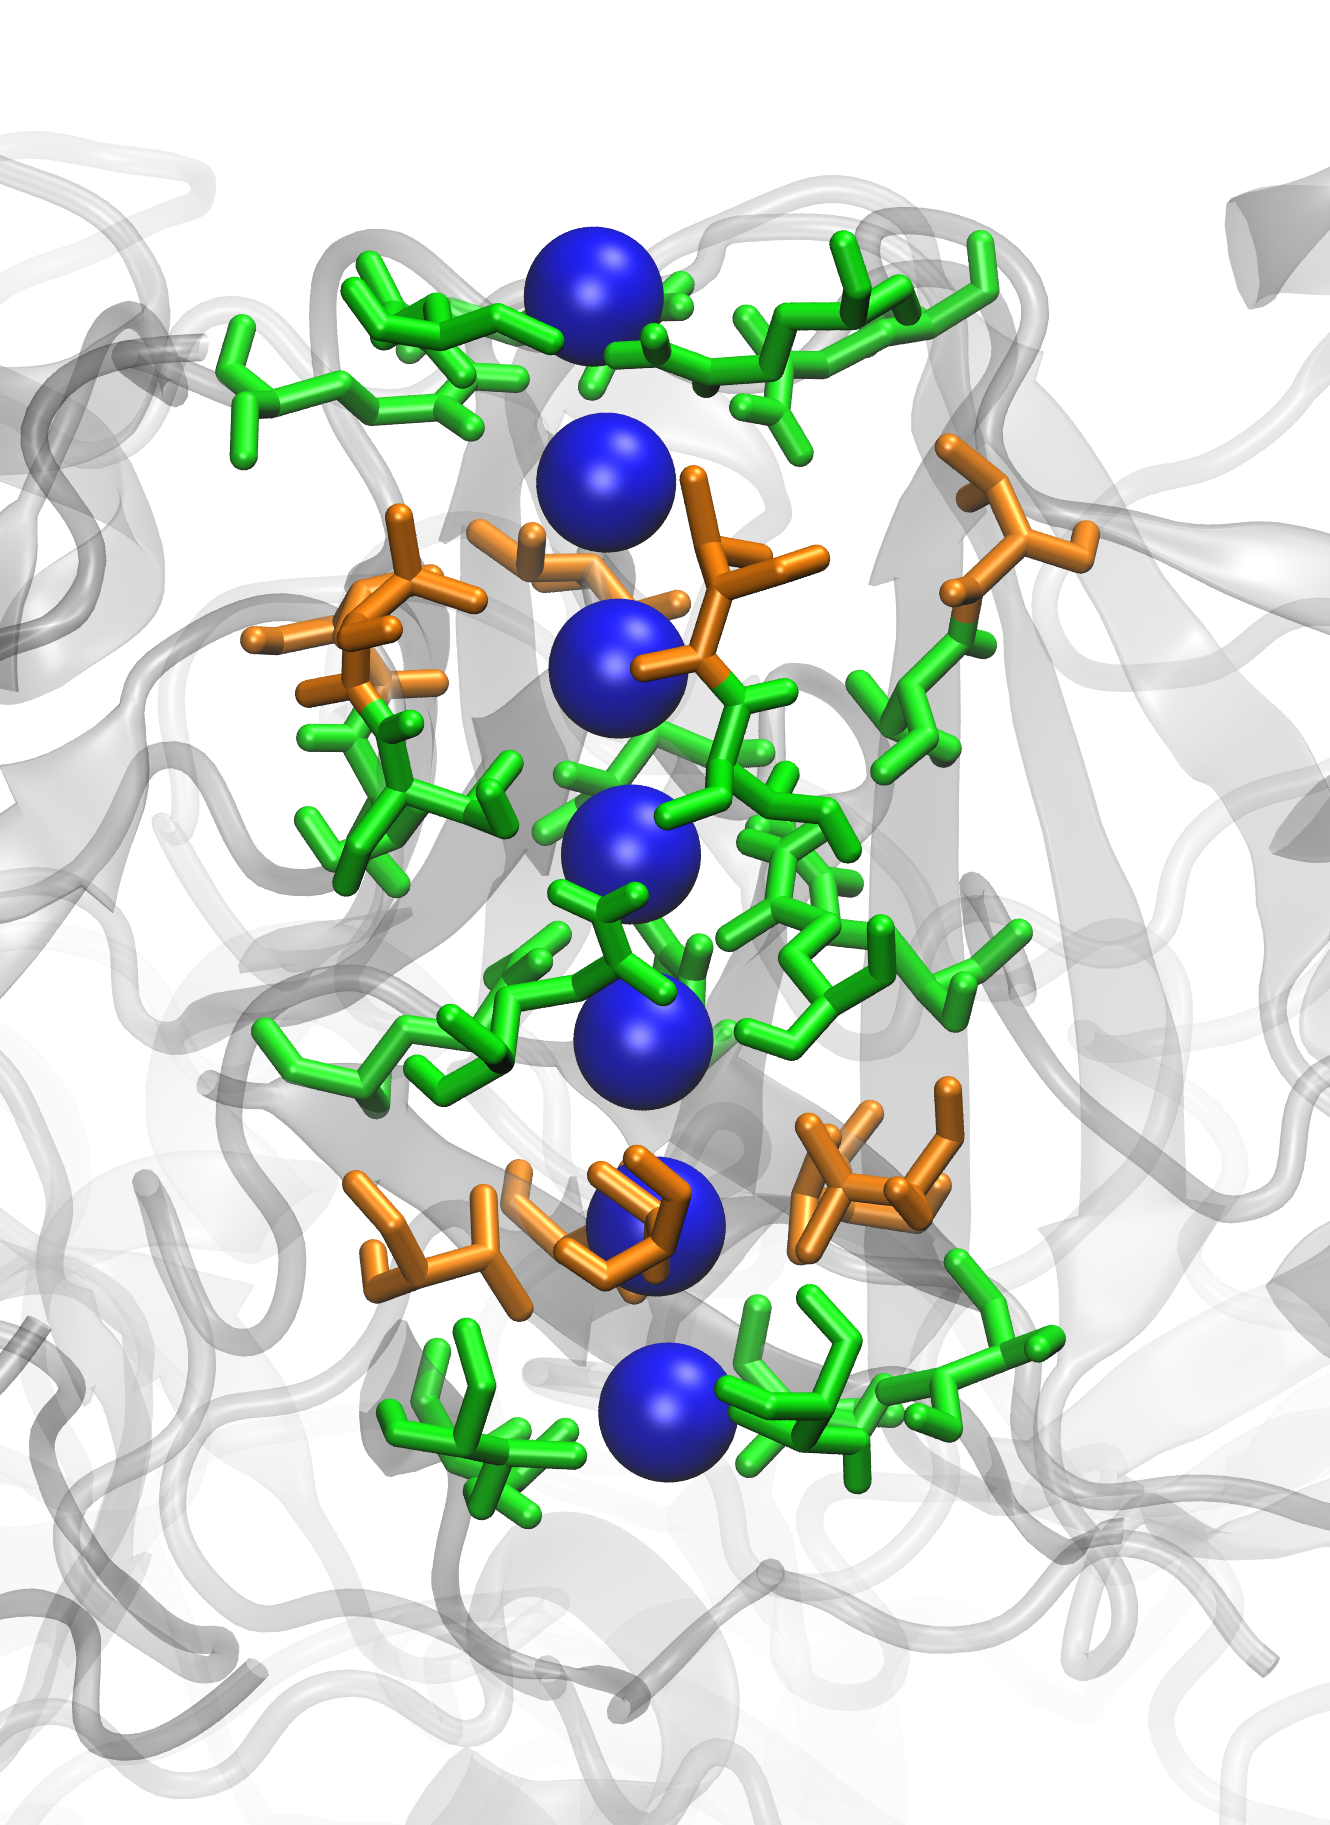
\includegraphics[width=0.6\textwidth]{Figure/TrV_pmf.png}
\end{figure}
}
\end{columns}

% \onslide<4->{
% \begin{minipage}[t]{0.4\textwidth}
% \centering
% \large
% \tikzmarkin<4->[set fill color=green!10, set border color=green]{pmf2}(1,-0.5)(0,0.5)
% Potencial de Fuerza Media\\ o\\ \textbf{PMF}\\
% $+$\\
% Umbrella Sampling
% \tikzmarkend{pmf2}
% \end{minipage}
% }
% \onslide<5->{
% \begin{minipage}{0.4\textwidth}
% \begin{figure}[ht]
% 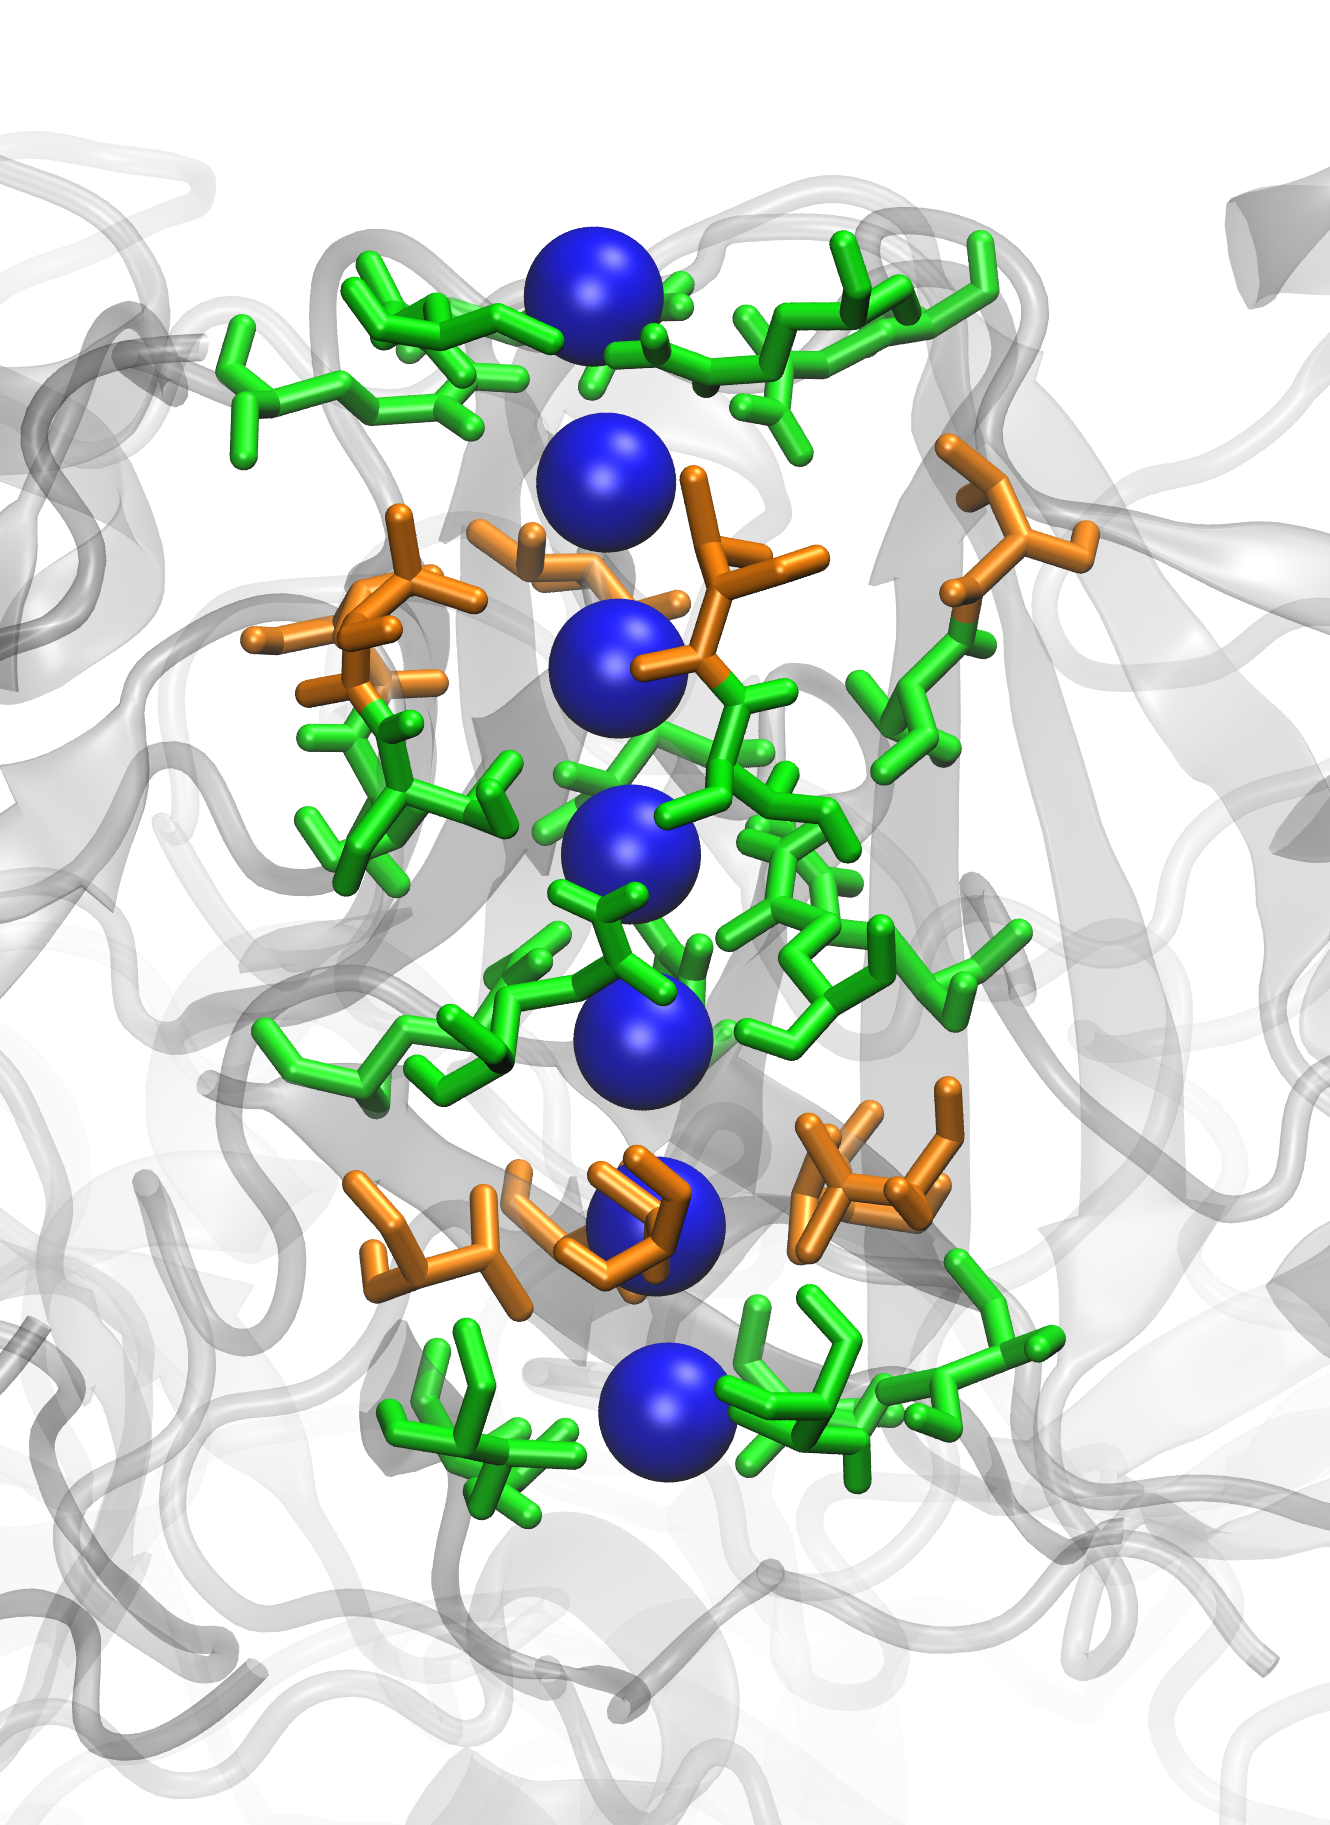
\includegraphics[width=0.9\textwidth]{Figure/TrV_pmf.png}
% \end{figure}
% \end{minipage}
% }
\end{frame}

\subsection{Perfil de Energía Libre en el poro de TrV}
\begin{frame}{Perfil de Energía Libre en el poro de TrV}
\begin{figure}[ht]
  \centering
  %\vspace{-0.25cm}
  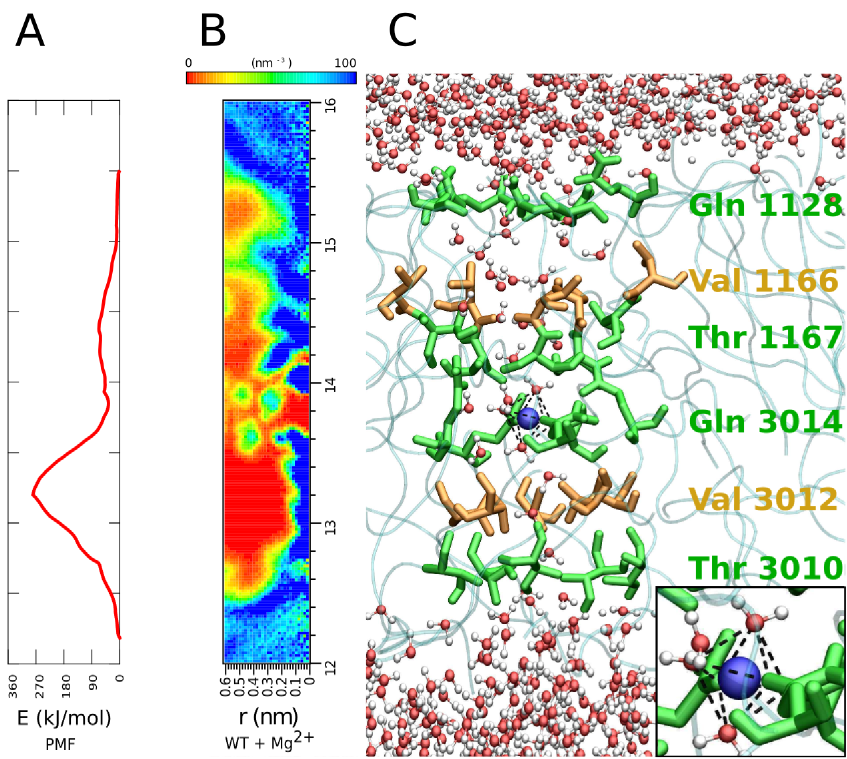
\includegraphics[height=6.3cm,keepaspectratio]{Figure/TrV_Mg_Dens.png}
\caption*{(A) Energía Libre de Gibbs del Mg$^{2+}$ en función de la coordenada de reacción. (B) Mapa de densidad de moléculas de agua (C) Vista lateral del poro de TrV.} %
\end{figure}
\end{frame}

\subsection{Conclusión II}
\begin{frame}{Conclusión II}
\begin{itemize}
    \item La presencia de un ion Mg$^2+$ en el poro a nivel de las Glutaminas 3014 logra la completa hidratación del poro.\vfill
    \item El perfil de energía libre nos indica que el ingreso de los iones ocurre desde el exterior de la cápside ya que de lo contrario, lo iones deberían atravesar una barrera energética mayor.\vfill
    \item La cadena continua de aguas podrían indicar la existencia de una cadena transportadora de protones.
\end{itemize}
\end{frame}

%
% Otros Virus
%

\section{Otros Virus}
\subsection{Puerta Hidrofóbica en otros Virus}
\begin{frame}{Puerta Hidrofóbica en otros Virus}
\hspace{-0.7cm}
\begin{minipage}[t]{0.4\textwidth}
\begin{itemize}
    \item<1-> Picornavirus.
    \begin{itemize}
    \item<1-> Human Rhinovirus 16.
    \item<2-> Poliovirus.
    \item<3-> Hepatitis A Virus.
    \end{itemize}
    \item<4-> Dicistrovirus.
    \begin{itemize}
    \item<4-> Cricket Paralysis Virus.
    \item<4-> Triatoma Virus.
    \end{itemize}
    \item<5-> Secovirus.
    \begin{itemize}
    \item<5-> Bean Pod Mottle Virus.
    \item<6-> Tobacco Ringspot Virus.
    \end{itemize}
\end{itemize}
\end{minipage}
\begin{minipage}[t]{0.6\textwidth}
\only<1>{
\begin{figure}[ht]
  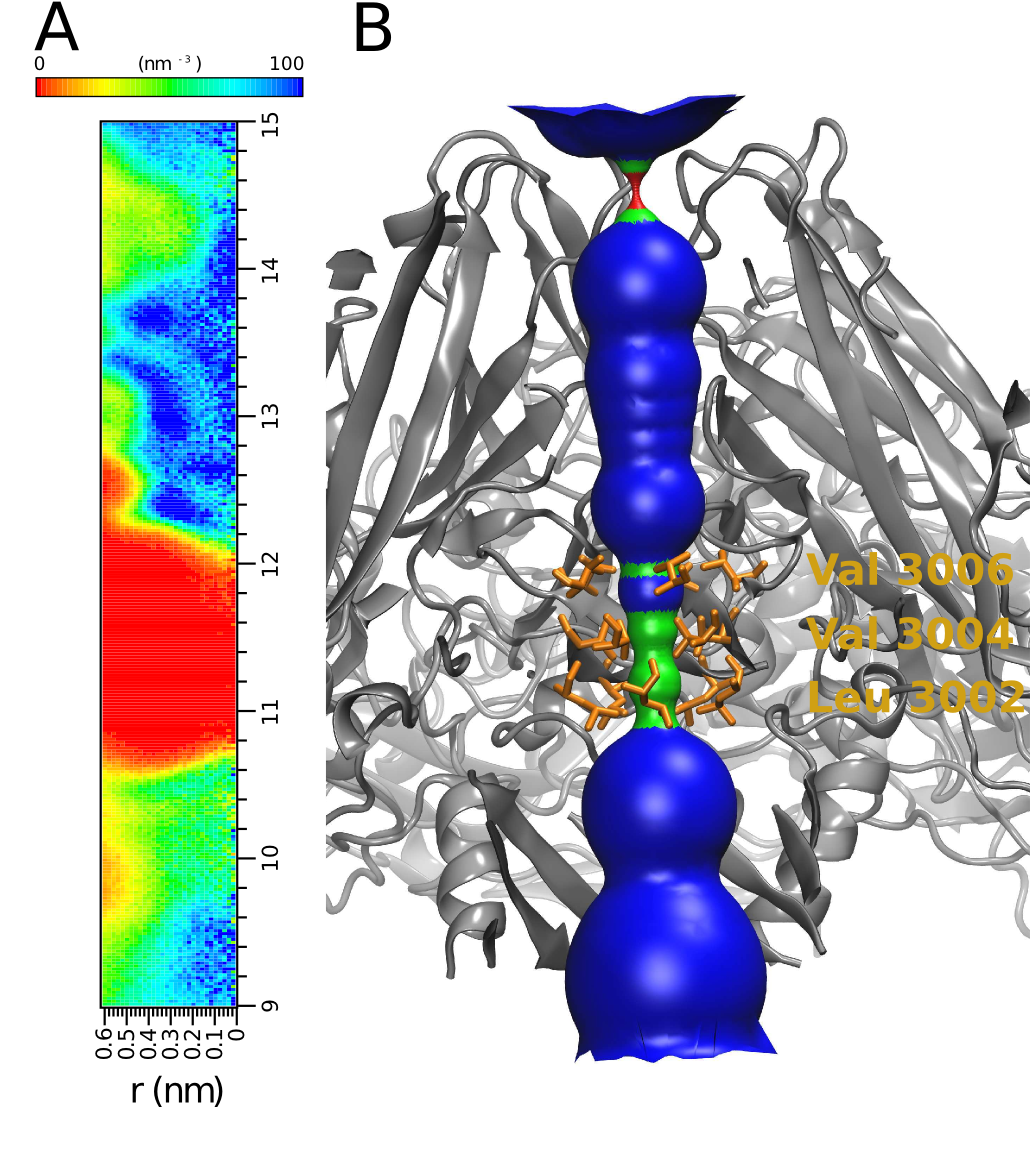
\includegraphics[height=7cm,keepaspectratio]{Figure/HRV16_Densmap.png}
\end{figure}
}
\only<2>{
\begin{figure}[ht]
  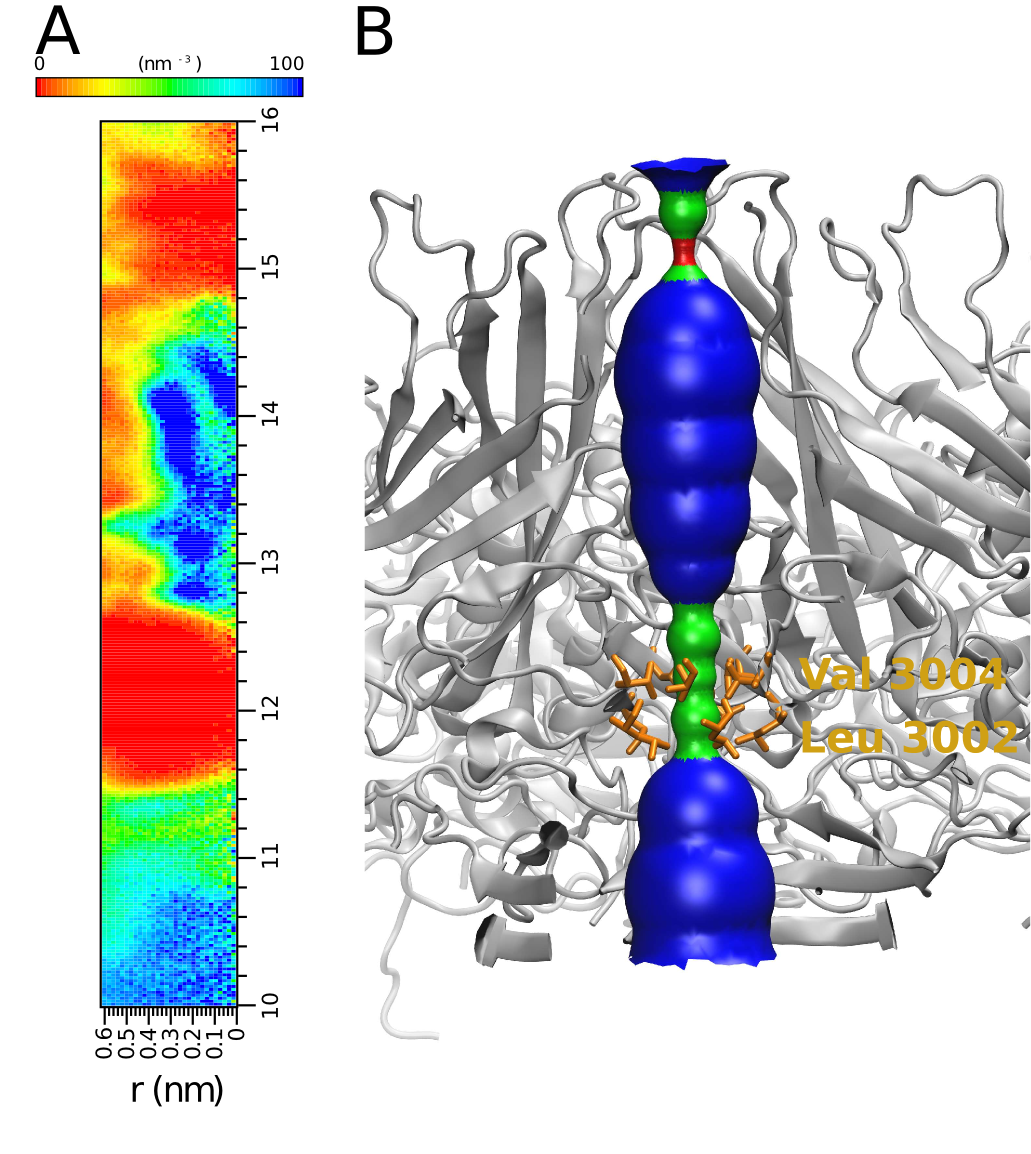
\includegraphics[height=7cm,keepaspectratio]{Figure/PoV_Densmap.png}
\end{figure}
}
\only<3>{
\begin{figure}[ht]
  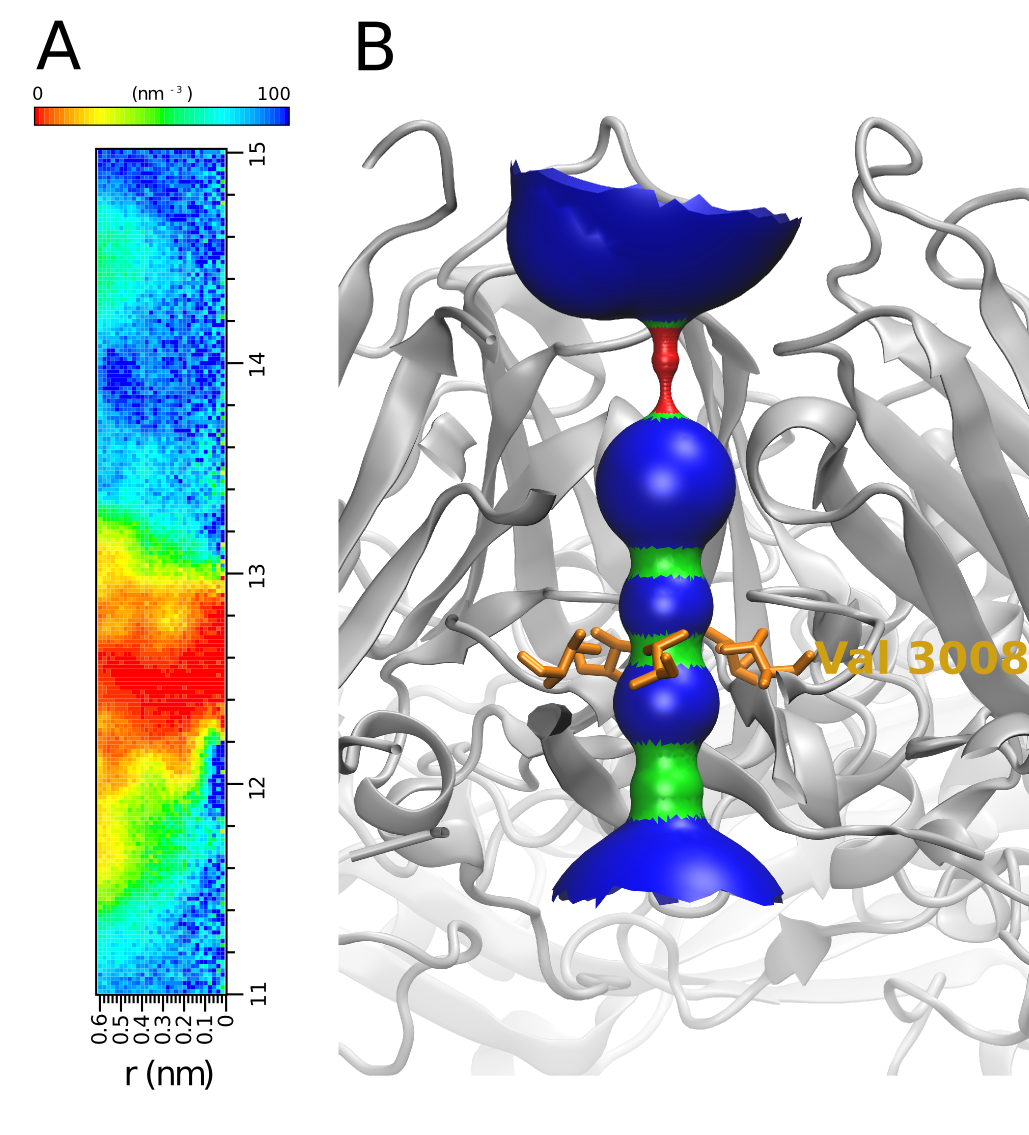
\includegraphics[height=7cm,keepaspectratio]{Figure/HAV_Densmap.png}
\end{figure}
}
\only<4>{
\begin{figure}[ht]
  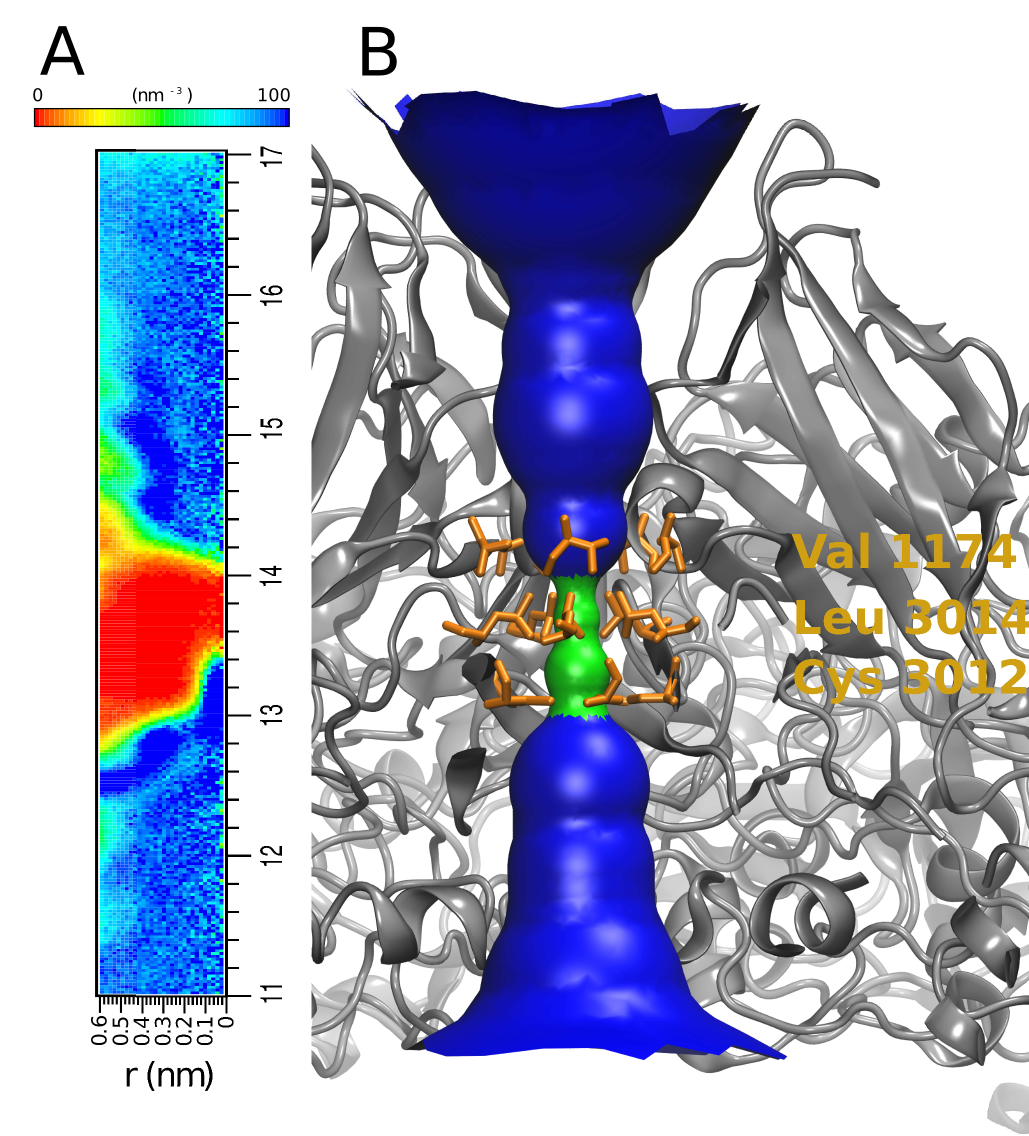
\includegraphics[height=7cm,keepaspectratio]{Figure/CrPV_Densmap.png}
\end{figure}
}
\only<5>{
\begin{figure}[ht]
  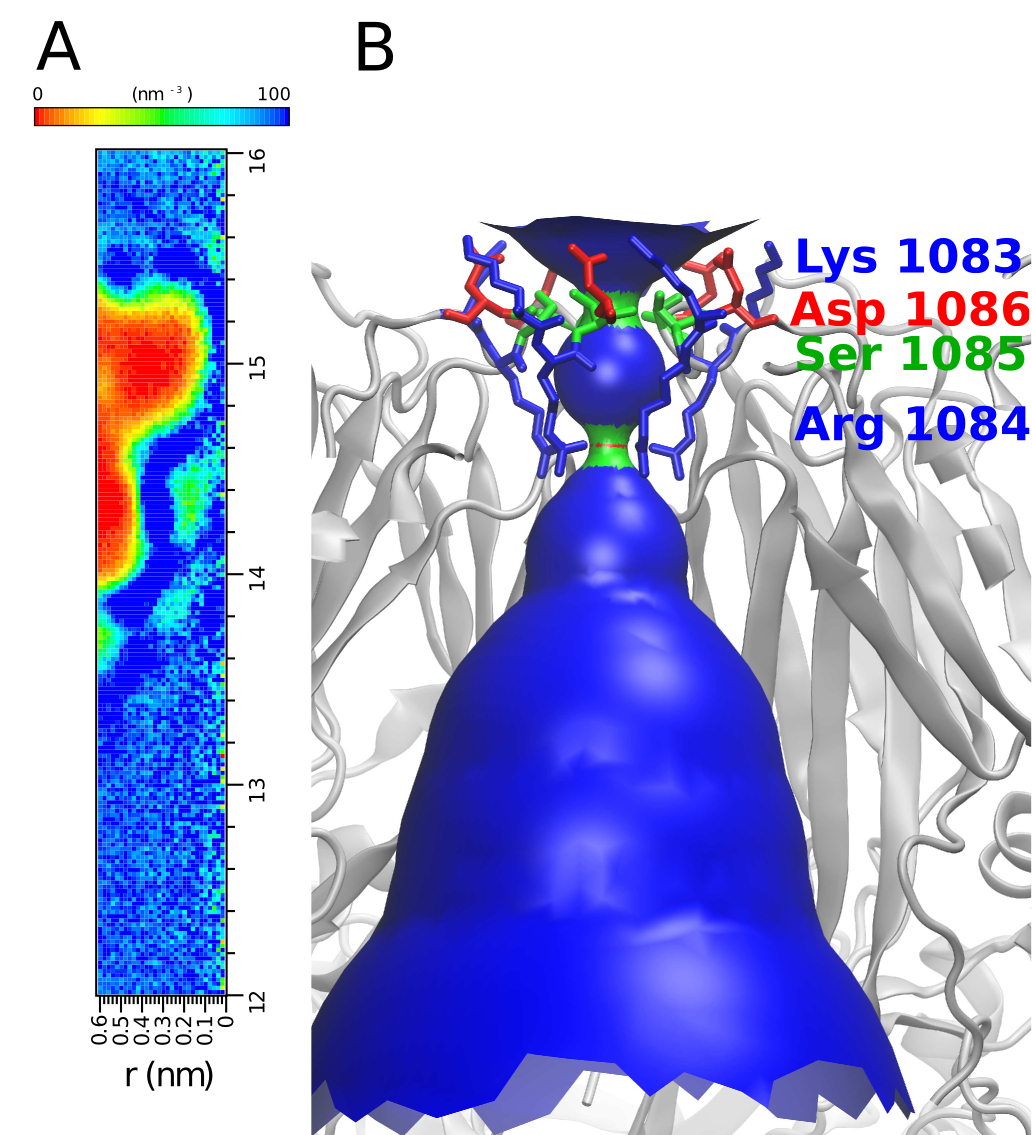
\includegraphics[height=7cm,keepaspectratio]{Figure/BPMV_Densmap.png}
\end{figure}
}
\only<6>{
\begin{figure}[ht]
  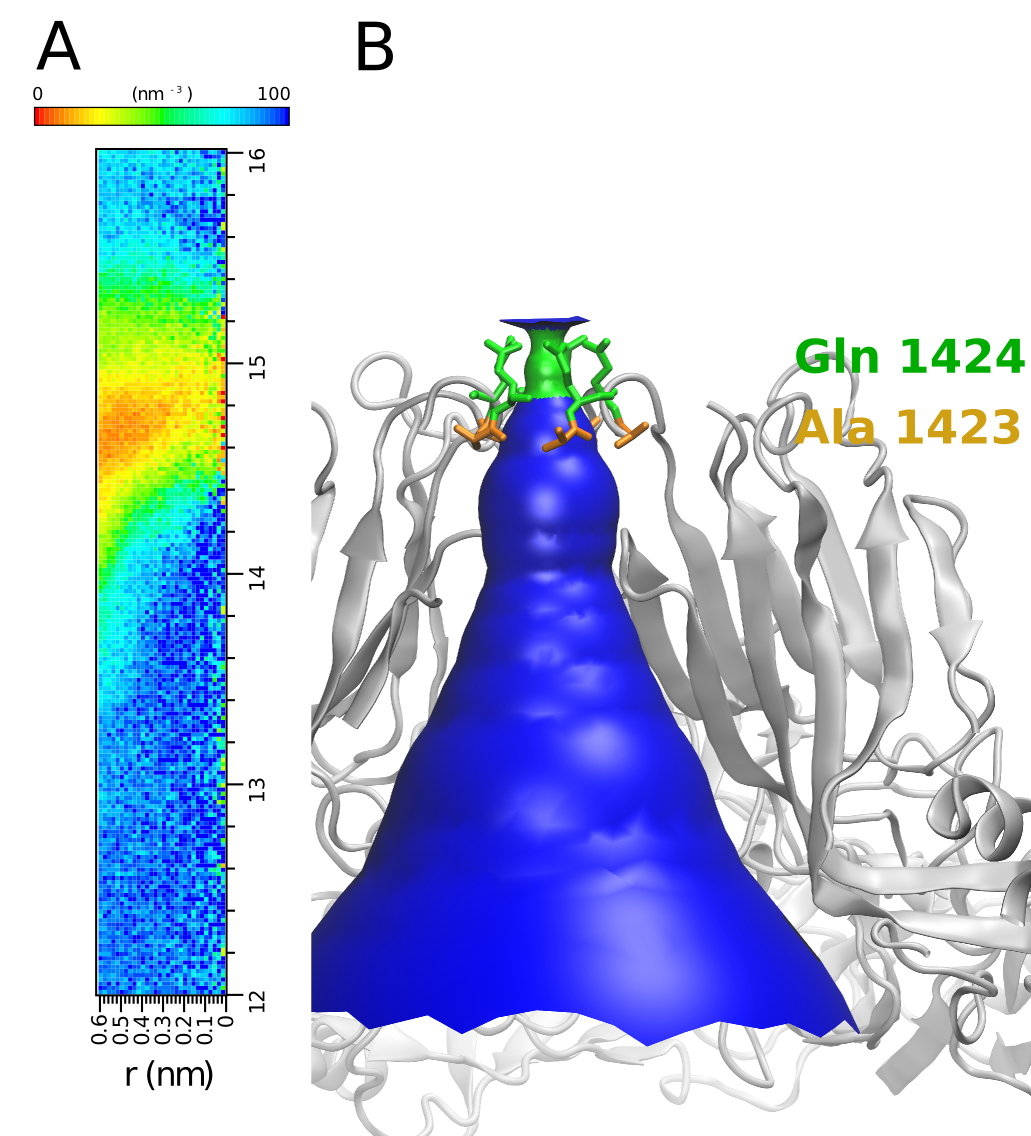
\includegraphics[height=7cm,keepaspectratio]{Figure/TRsV_Densmap.png}
\end{figure}
}
\end{minipage}
\end{frame}

\subsection{Conclusión III}
\begin{frame}{Conclusión III}
\begin{itemize}
    \item Los virus pertenecientes al orden \textit{Picornavirales} que infectan a animales (\textit{Picornavirus}) e insectos (\textit{Dicistrovirus}), presentan un mecanismo de regulación de apertura del poro presente en el eje quíntuple por medio de una puerta hidrofóbica.\vfill
    \item Los virus de la familia \textit{Secovirus}, que infectan a vegetales, no presenta el mismo mecanismo de puerta hidrofóbica.
\end{itemize}
\end{frame}

%
% Conclusión
%

\section{Conclusión}
\begin{frame}{Conclusión}
El objetivo de este trabajo consistió en responder las preguntas: ¿Existe algún
mecanismo de transporte en el eje quíntuple del Virus del Triatoma? Y de ser así, ¿De
qué manera regula su apertura? y ¿Qué tipo de moléculas son capaces de atravesarlo?
Teniendo en cuenta todo lo expuesto, se concluye que:
\begin{itemize}
\item<2-> El Virus del Triatoma presenta un poro en su eje quíntuple capaz de regular su apertura (Hidratación) a través de una puerta hidrofóbica ubicada a la altura del anillo de aminoácidos formado por las Valinas 3012.
\item<2-> La inserción de un ion Mg$^2+$ en el poro y su consecuente interacción con las Glutaminas 3014 ubicadas dentro del poro provocan la completa hidratación del poro. De esta manera, se logra la apertura del poro.
\item<2-> La formación de una cadena continua de moléculas de agua desde el exterior de la cápside hasta su interior podría indicar la existencia de un mecanismo de transporte de protones.
\end{itemize}
\end{frame}

\begin{frame}[t]{Palabras Finales}
\hspace{-0.5cm}
\begin{minipage}[t]{0.6\textwidth}
\centering
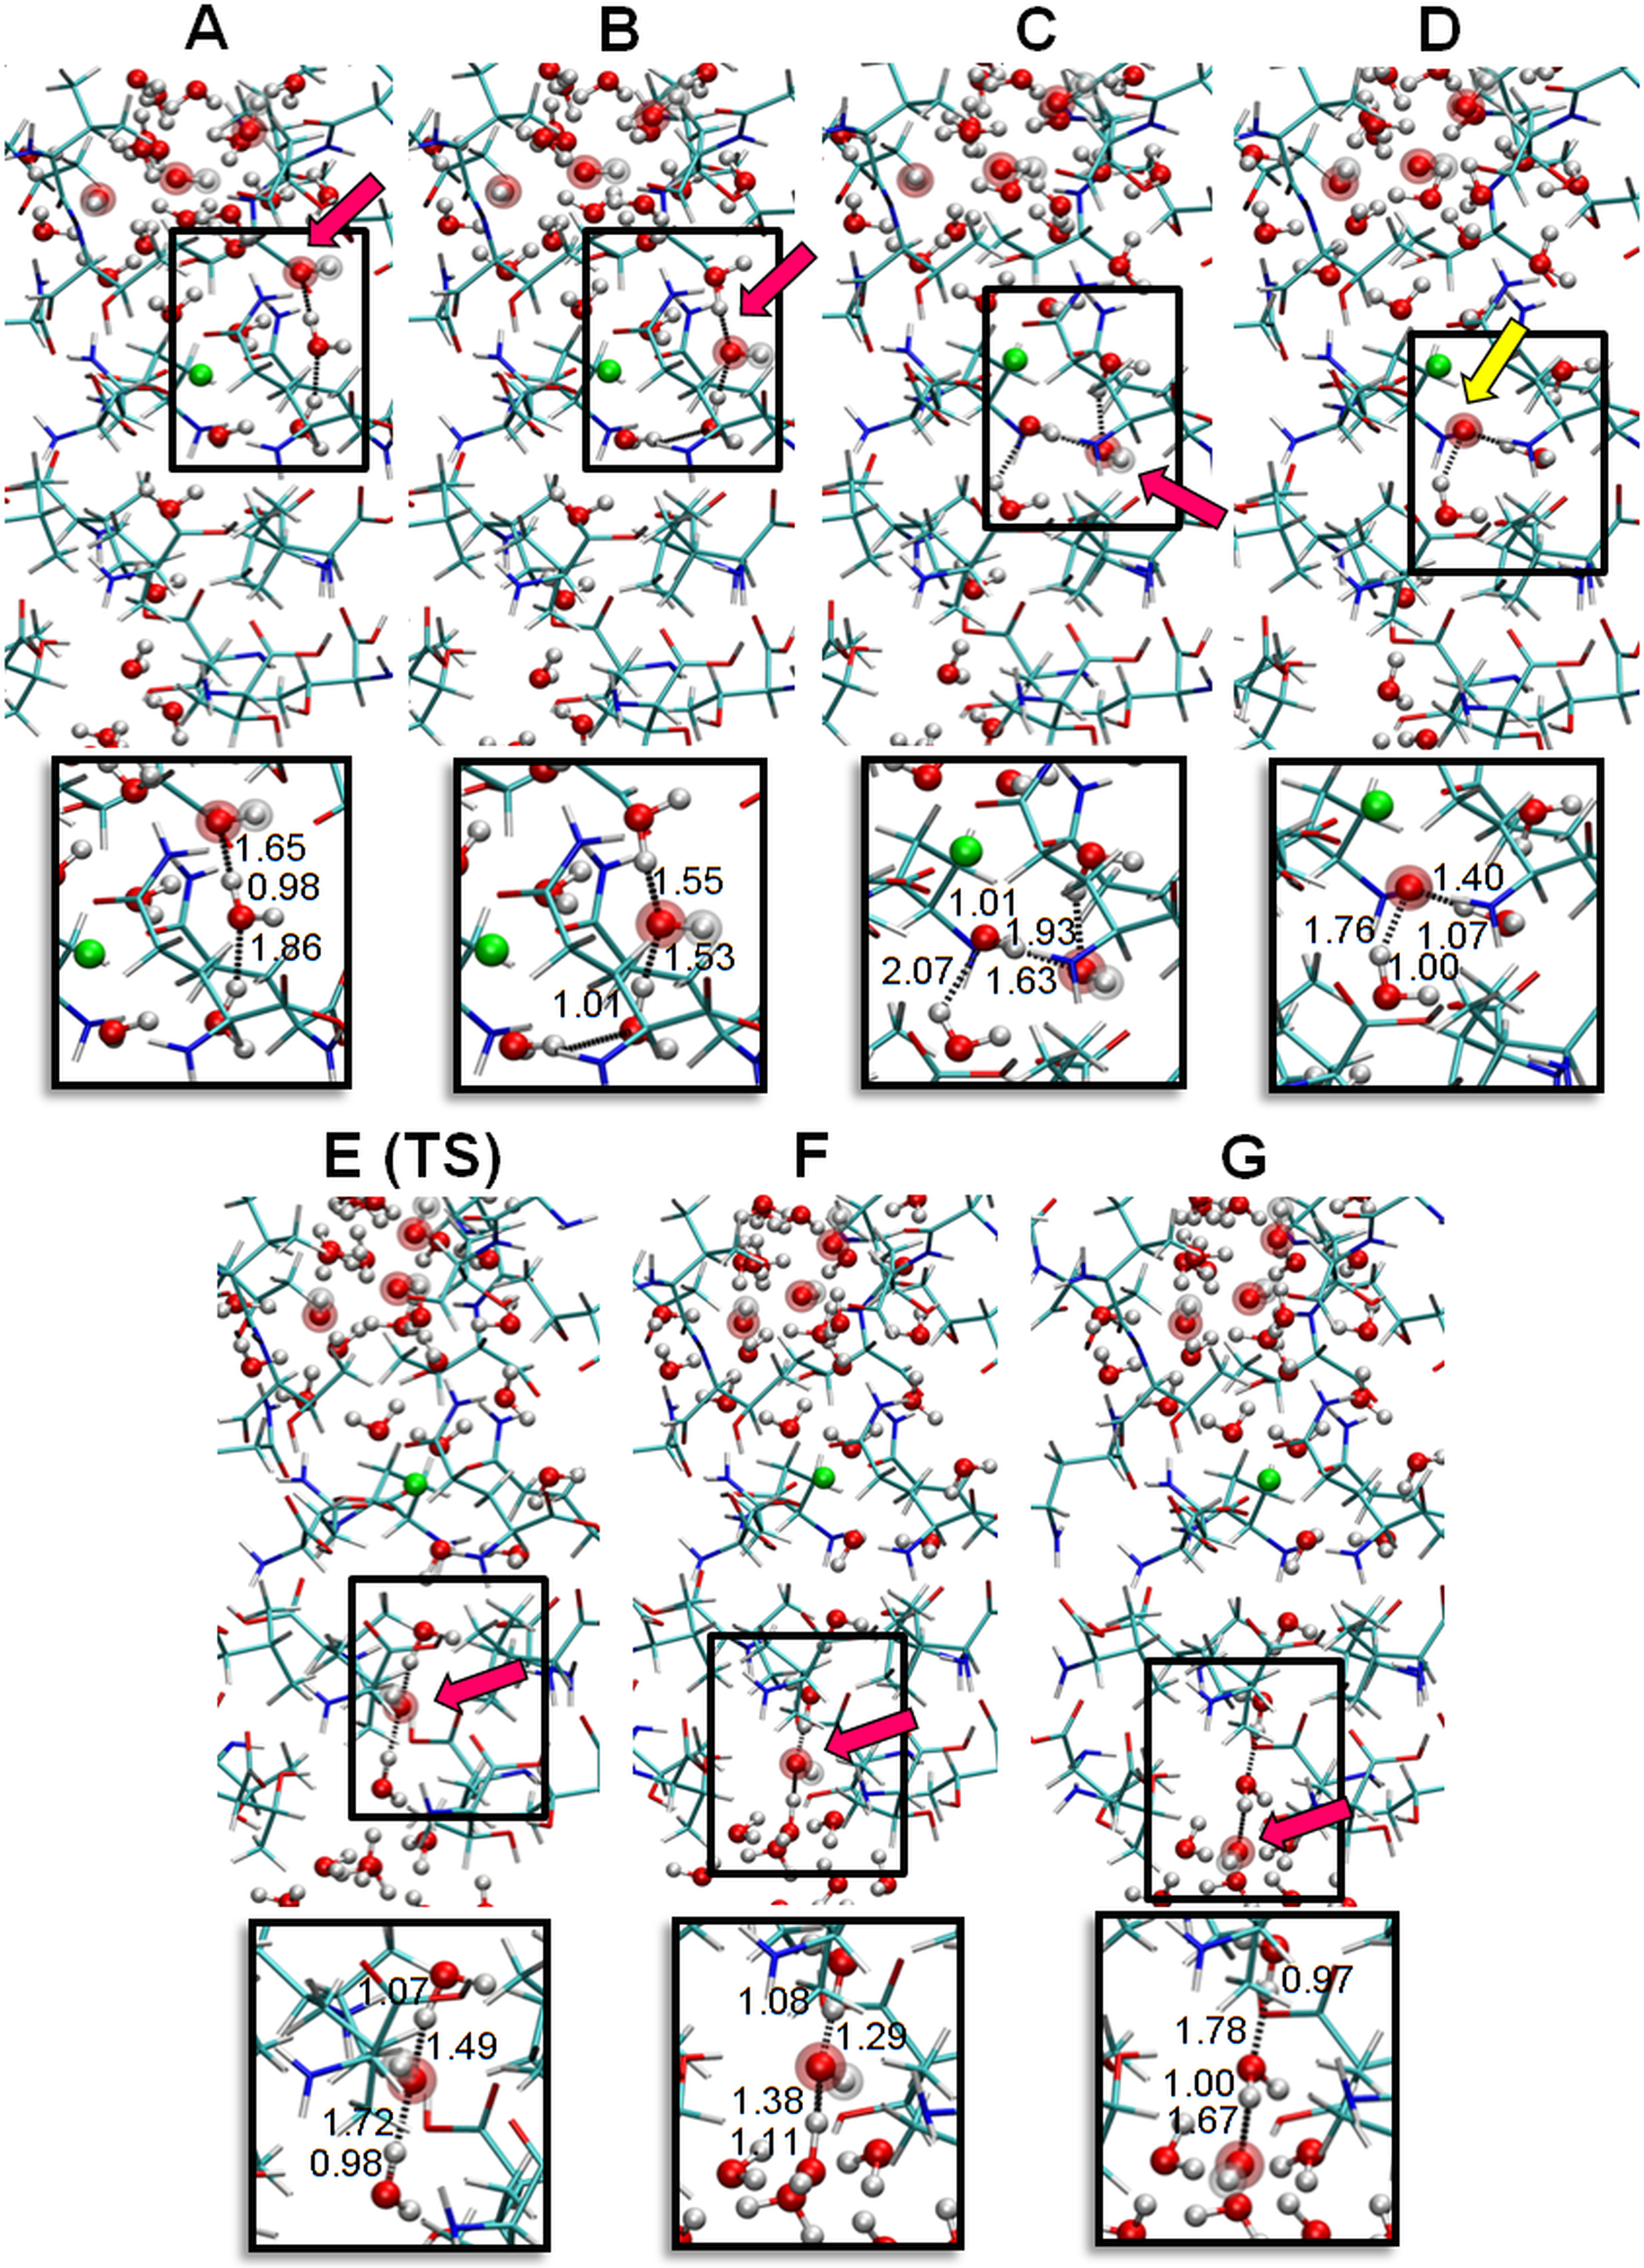
\includegraphics[height=7cm]{Figure/grothuss.png}
\end{minipage}
\begin{minipage}[t]{0.4\textwidth}
\centering
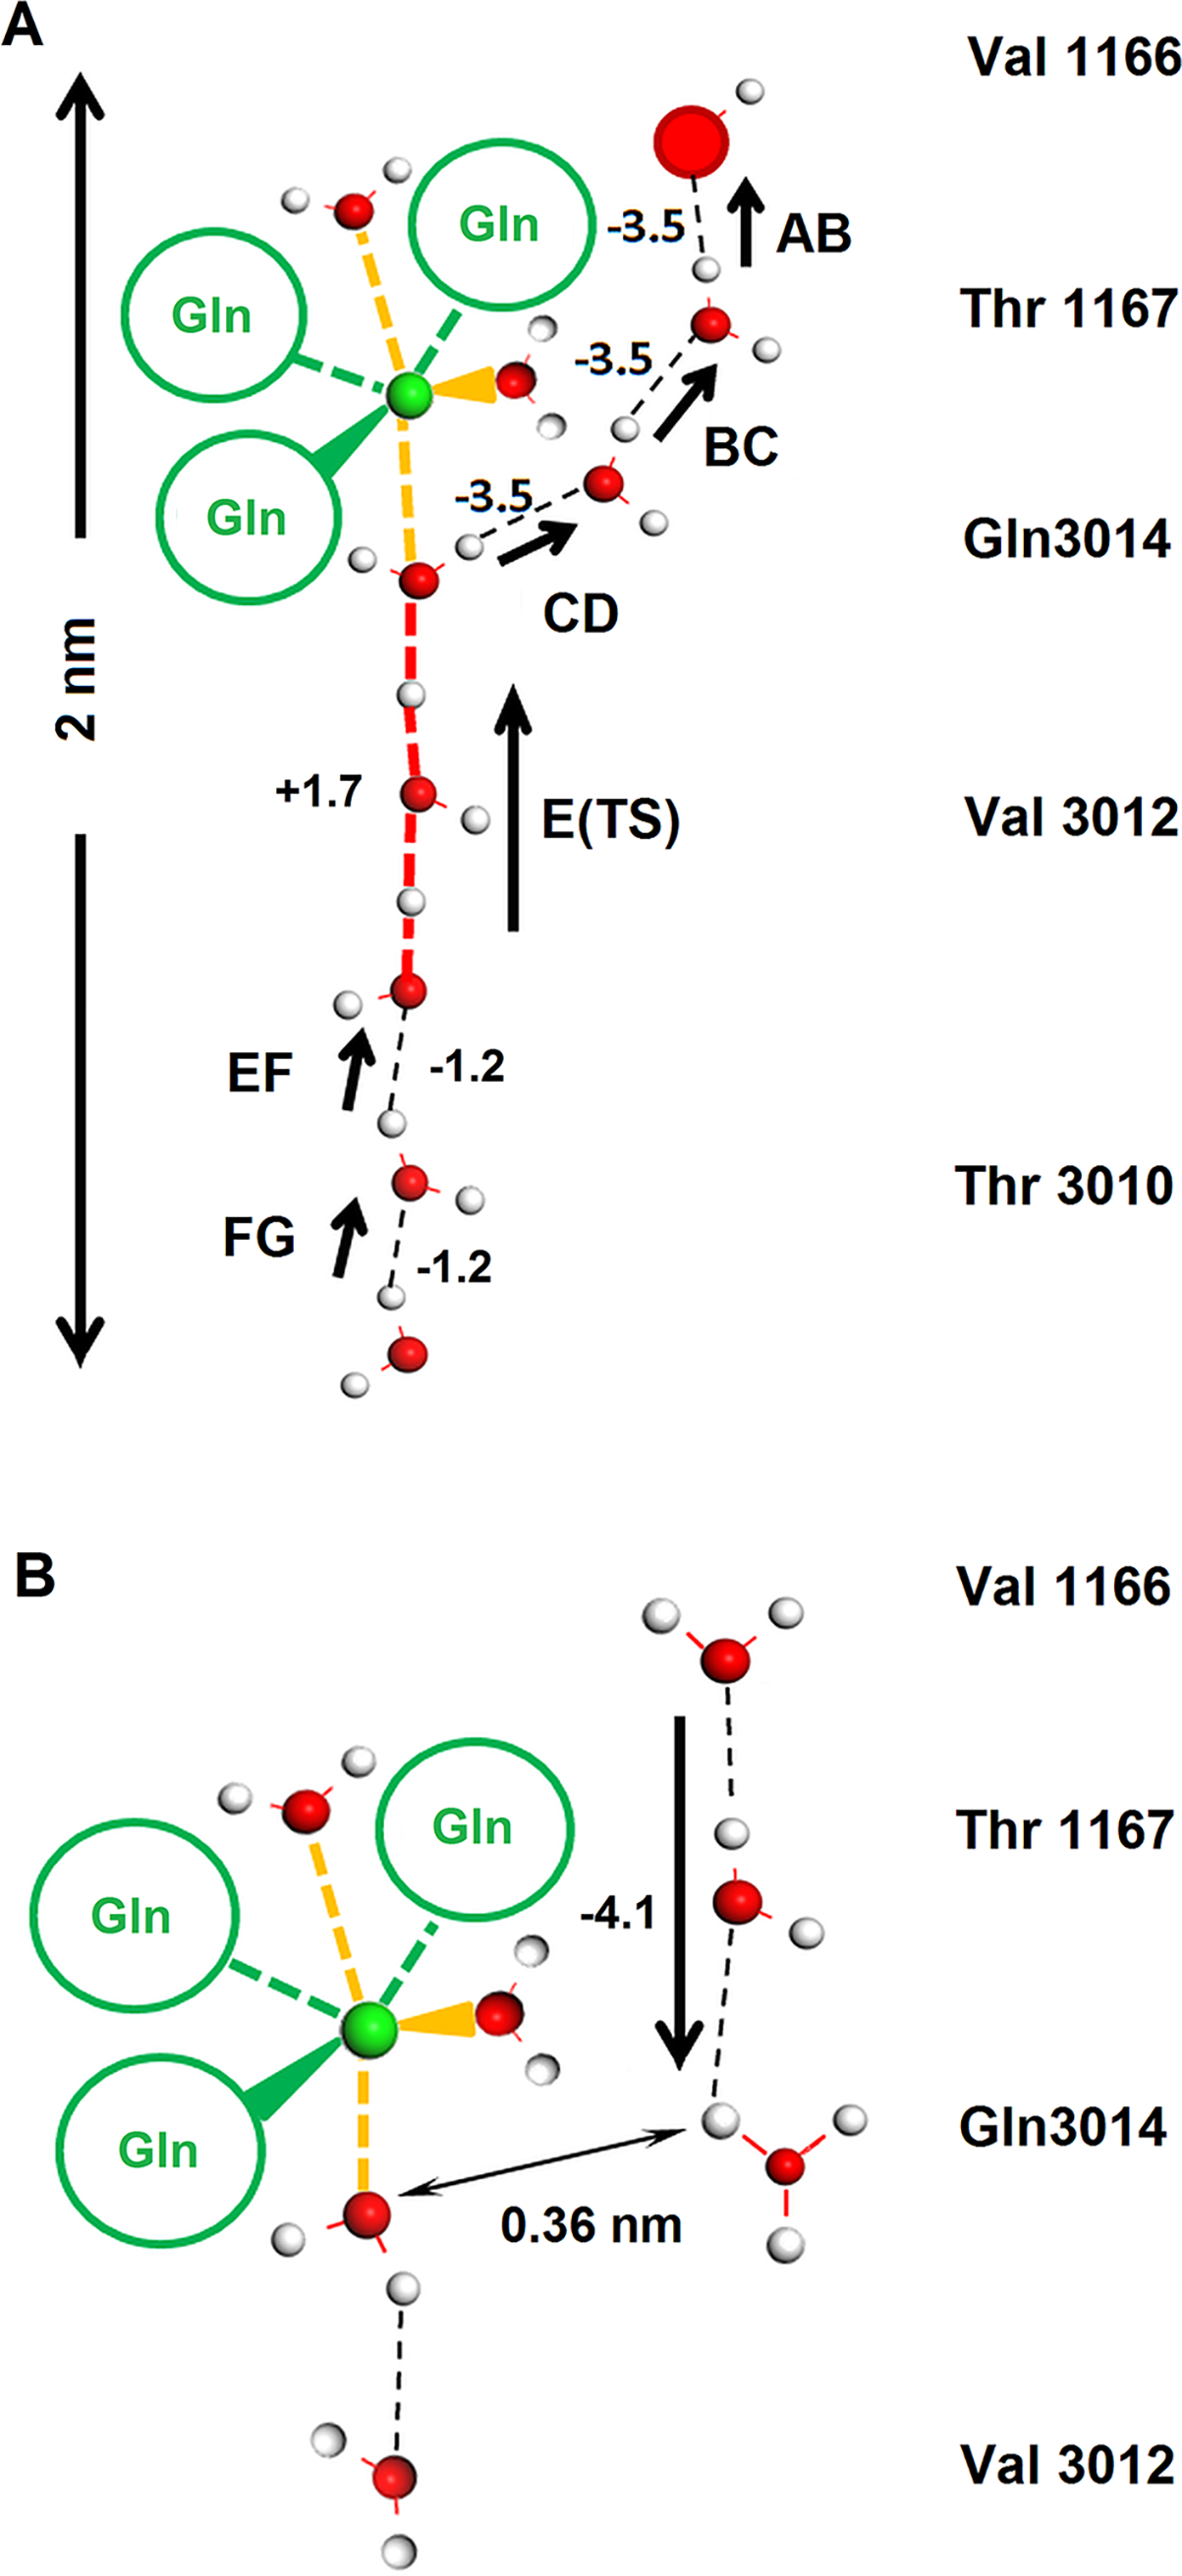
\includegraphics[height=7cm]{Figure/grothuss_2.png}
\end{minipage}
\end{frame}

\begin{frame}[t]{Palabras Finales}
\centering
\includegraphics[height=7cm]{Figure/paper.png}
\end{frame}

\begin{frame}[t]{Agradecimientos}
\small
\begin{itemize}
    \item<1-> Al departamento de Física de la UNS y al Instituto de Física del Sur por formarme y darme los medios para realizar este doctorado.
    \item<2-> A mi director, \textbf{Marcelo}, por introducirme en el mundo de la investigación.
    \item<3-> A mis compañeros de oficina, que me soportaron todo el doctorado. A \textbf{Fernando} que me enseño todo lo que sabia y me ayudo en los primeros pasos de este viaje.
    \item<4-> A \textbf{Nestor}, por sus charlas de ciencia, educación y otros temas.
    \item<5-> A \textbf{Sebastian} y \textbf{Michellina}, que me ayudaron y formaron como docente. A todos los integrantes de Curiosos. A todos los compañeros de cátedra.
    \item<6-> A \textbf{Ilan} y \textbf{Nadia} por transitar este camino juntos y ayudarnos mutuamente aunque sea solo prestando la oreja. A todos los que pasaron por la ofícina de becarios.
    \item<7-> A mis amigos de la universidad, \textbf{Duilio}, \textbf{Pau}, \textbf{Cris} y \textbf{Licho}, por su amistad y por aguantarme en todo este viaje.
    \item<8-> A \textbf{Maju}, hicimos todo este camino juntos y no se si lo hubiera terminado sin su amistad.
    \item<9-> A mis amigos de la infancia, \textbf{Rober}, \textbf{Seba}, \textbf{Gaspar}, \textbf{Fede} y \textbf{Sonia}, después de
tanto tiempo siempre presentes.
    \item<10-> Por último y más importante a mi \textbf{Familia}. A mis \textbf{Padres} por darme todo. A mis
\textbf{Hermanos}, a pesar de las peleas, siempre apoyándome.
    \item<11-> A \textbf{Jobo}.
\end{itemize}
\end{frame}

\end{document}